\documentclass[]{report}

\usepackage[backend=biber,style=numeric,sorting=none]{biblatex}
\usepackage{amsmath,amssymb,amsfonts}
\usepackage{graphicx}
\usepackage{textcomp}
\usepackage{xcolor}
\usepackage{todonotes}
\usepackage[margin=1in]{geometry}
\usepackage{fancyhdr}
\usepackage{titlesec}
\usepackage{float}
\titleformat{\chapter}[display]
  {\normalfont\bfseries}{}{0pt}{\Huge}

\def\c#1{\texttt{#1}}

\bibliography{bibliography}
\pagestyle{fancy}
\fancyhf{}
\rhead{150010440}
\lhead{CS4099 Senior Honours Project Report}
\rfoot{You know we on page \thepage{} now son}

\begin{document}

\title{SH Project Report}
\author{Cameron Allan}

\begin{titlepage}

\newcommand{\HRule}{\rule{\linewidth}{0.5mm}}
\renewcommand{\contentsname}{Table of Contents}

\center
 
%----------------------------------------------------------------------------------------
%   HEADINGS
%----------------------------------------------------------------------------------------

\textsc{\LARGE University of St Andrews}\\[1.5cm]
\textsc{\Large CS4099}\\[0.5cm]
\textsc{\large SH Project Report}\\[0.5cm]

%----------------------------------------------------------------------------------------
%   TITLE
%----------------------------------------------------------------------------------------

\HRule \\[0.4cm]
{ \huge \bfseries An online card-based game to explore human response to predefined scenarios}\\[0.4cm] % Title of your document
\HRule \\[1.5cm]
 
%----------------------------------------------------------------------------------------
%   AUTHORS
%----------------------------------------------------------------------------------------

\begin{minipage}{0.4\textwidth}
\begin{flushleft} \large
\emph{Author:}\\
Cameron \textsc{Allan}
\end{flushleft}
\end{minipage}
~
\begin{minipage}{0.4\textwidth}
\begin{flushright} \large
\emph{Supervisor:} \\
Dr. Ruth \textsc{Letham}
\end{flushright}
\end{minipage}\\[0.5cm]

{\large \today}\\[0.5cm]


\includegraphics[scale=0.5]{images/st-andrews-shield.png}

\vfill
\end{titlepage}

\tableofcontents

\newpage

\begin{abstract}
    There are many situations in which it is desirable to know the opinions of a population. Aside from standard opinion surveys, little to no research has been done into alternative methods of gathering the public opinion. 

    This project was undertaken in collaboration with the St Andrews Centre for Exoplanet Science\cite{CfES}, in an attempt to develop a software artifact capable of capturing user decisions in a game interface. This project focuses on the framework through which these games may be created, played and visualised, with the end goal of analysing these responses and inferring user's opinions on certain subject matters through their choices. The framework is designed to be highly flexible, allowing all aspects of a game's story and development to be decided by an administrator.
\end{abstract}

\chapter{Declaration}
    I declare that the material submitted for
    assessment is my own work except where credit is
    explicitly given to others by citation or
    acknowledgement. This work was performed during
    the current academic year except where otherwise
    stated.

    The main text of this project report is \todo[inline]{Add word count} NN,NNN* words long, including project specification and plan.

    In submitting this project report to the University of
    St Andrews, I give permission for it to be made
    available for use in accordance with the regulations of
    the University Library. I also give permission for
    the title and abstract to be published and for copies of
    the report to be made and supplied at cost to any bona
    fide library or research worker, and to be made
    available on the World Wide Web. I retain the
    copyright in this work.

\chapter{Introduction}

\section{Motivation}
This project is undertaken in collaboration with the St Andrews Centre for Exoplanet Science, with an aim to answer the question; how would the general human population react to the discovery of alien life?
There has been research~\cite{ReactionsToMessage, HowReactDiscovery, Fear} into this area, but it is certainly not extensive and very little of it is systematic. The topic is vast, and is made more complex by many factors that may affect the answer:
\begin{itemize}
    \item How has extra-terrestrial life been discovered?
    \item What is the nature of the life, is it intelligent?
    \item Is alien life on our doorstep, or far enough away that it could never reach or harm us?
\end{itemize}
Anne Smith (Biology) and Christine Helling (Astronomy) of the St Andrews Centre for Exoplanet Science believe it could be beneficial to create a game capable of collecting answers to questions like these. Gamification has been used in many areas, and has been shown to consistently improve engagement~\cite{engage}. Hopefully, this format of gathering opinions would allow participants to become immersed in the context of the quesiton, hopefully leading to more honest responses. 

If it was possible to accurately capture players' thoughts and feelings in this manner, this could impact the way opinion data is collected across multiple faculties.

\section{Achievements}
The framework created for this project can be conceptualised as three distinct sections:
\begin{itemize}
    \item Game Interface
    \item Game Maker
    \item Visualisation
\end{itemize}
The game interface provides the portal through which participants can play games built and stored on the platform. The game maker provides an interface through which an administrator may create games, and edit those previously made. Finally, the visualisation tools allow administrators to filter and visualise how players interact with the game.

\section{Document Outline}
After outlining the objectives of this project, this document reviews the software and literature surrounding gamification - the main topic with which this project is concerned.
Coevered then are the processes followed, tools used and considerations taken into account when designing, implementing and testing the framework. 
Following this, an analysis of testing and user evaluation.
Finally, the software is evaluated with respect to the objectives.

\section{Objectives}
As part of my Description, Objectives, Ethics and Resources (DOER) document I described the objectives of this project. Over the course of the project, they remained the same apart from one change - making~\ref{SO:2} a secondary objective, rather than primary. This was done as the focus of the project shifted towards creating an unbiased framework, while this objective was content-focused and so became lower priority.

\subsection{Primary Objectives}
\begin{enumerate}[label=\textbf{PO.\arabic*}]
    \item Devise and implement a game that presents the player with scenarios and allows them to choose from potential responses
    \item Devise and implement a flexible infrastructure to model and constrain scenarios and their impacts
    \item Devise and implement an infrastructure for capturing and recording player responses
    \item Implement basic visualisation of responses
\end{enumerate}
\subsection{Secondary Objectives}
\begin{enumerate}[label=\textbf{SO.\arabic*}]
    \item Devise and implement an admin centre to allow easy creation of new game content
    \item \label{SO:2} In collaboration with Anne Smith and Christine Helling, devise a sample set of appropriate scenarios with impacts and populate the game
    \item Carry out an experiment to assess the effectiveness of the game as a tool to assess people's real world views
    \item Create more advanced visualisation and analysis tools
\end{enumerate}
\subsection{Tertiary Objectives}
\begin{enumerate}[label=\textbf{TO.\arabic*}]
    \item Perform a wider user experiment
\end{enumerate}

\section{Definitions}
Throughout this text I will use the following words defined as so:
\begin{itemize}
    \item Player/Participant - A user playing the game through the UI
    \item Administrator - An user that has access to the game maker and visualisation applications. This would be an individual interested in researching the opinions a group holds on a subject matter.
    \item Game definition - A game within the context of the framework I have created. A unique game definition consists of a set of cards, a set of pillars, and a starting deck
\end{itemize}
\chapter{Context Survey}

Here I will review the existing software and literature on the different aspects of this project. 
I will briefly look at the psychological and gamification aspects 
\todo{finish}

\section{Opinion of First Contact?}
As this project has been undertaken in collaboration with the Exoplanet Research Society, it is worth briefly reviewing the literature on the target question - how would humans react to the discovery of alien life? There has been some research\cite{ReactionsToMessage, HowReactDiscovery, Fear} into this area, but it is certainly not extensive and very little of it is systematic. The topic is vast with many variations:
\begin{itemize}
    \item How has extra-terrestrial life been discovered?
    \item What is the nature of the life, is it intelligent?
    \item Is alien life on our doorstep, or far enough away that it could never reach or harm us?
\end{itemize}
Anne Smith and Christine Helling believe it could be beneficial to create a game capable of collecting this information, in order to reduce the burden on participants answering such an extensive library of questions and improve engagement.
\todo{finish}

\section{Similar Software}
\todo{fill}

\section{Survey Gamification}
An emerging trend in modern business practice, gamification consists of `using game mechanics and game design elements to measure, influence and reward user behaviors.'~\cite{7804551}. 
There has been some research into gamification as a tool to improve the quality of responses from and engagement with surveys. 
The results of this research has been summarised by Briana Brownell, Jared Cechanowicz, and Carl Gutwin as follows: 
`In most cases, their results show that the addition of these game elements increases the length and quantity of responses, and respondents typically prefer the gamified version to the standard survey version. However, their research does not compare the effectiveness of game elements in gamified surveys. They have also found that that some gamified survey designs can lead to compromised respondent data (Puleston \& Sleep, 2011).'~\cite{SurveyGamificationResearch}.
This indicates that there is promise in the notion of gamifying surveys.
As noted by Brownell et al, however, gamification can result
\todo{finish}

Typically, the experiments discussed in the papers referenced only go as far as to change the wording of survey questions, show imagery or 
\todo{finish}

A 2011 paper found that while participants' enjoyment of the survey sees a great increase, there are three main effects that gamification has on the `character of the data'~\cite{GameExperiments}:
\begin{enumerate}
    \item Effects caused by changes to the question and how it is interpreted
    \item Effects caused by changing the attitude and mindset of respondents
    \item Effects caused by changes to the design and layout of question
\end{enumerate}
These are things I kept in mind while making design decisions, as if the software is to be used in an experiment, it's imperative that there is no bias inherent in the framework.

\section{Game Model}
\subsection{Reigns}
When proposing the format of the artifact, I based my framework on an existing game, Reigns~\cite{Reigns}. 
In Reigns, the player takes the role of a medieval ruler, and makes binary decisions to solve problems their subjects approach them with. 
These decisions affect further scenarios that may appear, as well as changing how the ruler is perceived by various factions, such as their population, army and church. 
The player's success is measured by how many decisions they can make without falling out of favour with any of the factions.

As of 2019-03-01, this is a well reviewed game, with a rating of 4.7/5 on the Google Play store~\cite{GooglePlay}. 
Given this, in addition to the simplicity of recording and analysing the choices, I believe the framework of Reigns could provide a good starting point for gathering player opinions. 

\chapter{Requirements}

\todo[inline]{Elaborate on requirements}

Below are the requirements that I specified early on in the project.

\section{Functional Requirements}

\begin{itemize}
        \item A user can enter a unique id, under which their game data will be recorded
        \item A user can choose a game to play by entering the game code
        \item A user can, read and respond to scenarios presented to them
        \item A user can see the effect that their responses have on the pillars
        \item A user can lose a game, when the value of one of their pillars reaches zero
        \item  An administrator can add, edit and remove cards from a game definition
        \item  An administrator can add, edit and remove pillars from a game definition
        \item  An administrator can view a summary of the game they are creating, which contains information on any machine detectable oversights and game balance 
        \item  An administrator can save a game they are editing and return to it later, or let users play it
        \item  An administrator can save their progress in editing one game and switch to another
        \item An administrator can select specific cards and obtain visualisations that summarise how players respond to them
        \item An administrator can filter turns included in visualisations by the state of the game during those turns
        \item An administrator can export and download all game data to an appropriate data processing format
\end{itemize}

\section{Non-Functional Requirements}

\begin{itemize}
    \item All interfaces are clear and intuitive
    \item The game interface is responsive to input - there should be minimal delay between an input action and the outcome
    \item The game interface does not influence the user's choice in a way that is not customisable
    \item User data should be stored securely
\end{itemize}
\chapter{Software Engineering Process}

As the majority of the work put into this project was in developing the software artifact, I focused from the beginning on following an effective software engineering process. This is detailed in Section~\ref{proc}. Section~\ref{tool} is closely related, describing the tools that enabled me to follow the process.

\section{Process}\label{proc}
I employed an agile\cite{Agile} methodology throughout my work on this project. 

One of the key Agile principles is to `Deliver working software frequently'\cite{AgileKey}. 
I followed this from the beginning by setting myself intermediary deadlines, by which I planned to demo working sections of project. 
These deadlines were discussed and agreed upon with my supervisor. 
This helped me stay focused on getting the features I needed working while avoiding premature optimisation.

Another primary principle of the Agile Manifesto is to `Welcome changing requirements, even late in development'\cite{AgileKey}. 
As an example of this, one of my original requirements involved assessing how accurately \od{} could gather people's real world views. 
After thinking more about the psychological aspects of this question, my supervisor and I decided that this was outside the scope of the project as it is closer to psychology than computer science. 
After realising this, we changed this requirement to performing a simple user evaluation. 

\section{Tools}\label{tool}
With this in mind, one of the first tools I employed was the version control system Git~\cite{Git}.
Given the size of the project, it was important to be able to revert the project to a previous point in case some functionality broke.
Version control software was the obvious solution, and Git is the one of these that I have the most experience with. To complement this, I set up a master GitHub~\cite{GitHub} repository to use as a backup.

In addition to serving as a backup, GitHub provides a useful set of project tracking features. 
I did consider other tools often used to track projects, such as Trello~\cite{Trello}, but in the end decided that GitHub's ability to reference aspects of the code (thanks to them being stored in the same place) made it better suited for my needs. 
Here I will outline the features that I used and describe how they helped my development process:

\paragraph{Issues} These are a core element of GitHub; any task that needs completing is documented as an issue.
I kept my issues fairly high-level, as I have found previously that too much detail in issues results in spending excessive amounts of time managing them or some inevitably become outdated. Figure~\ref{fig:issue} shows an example issue.

\begin{figure}[!h]
	\centering
	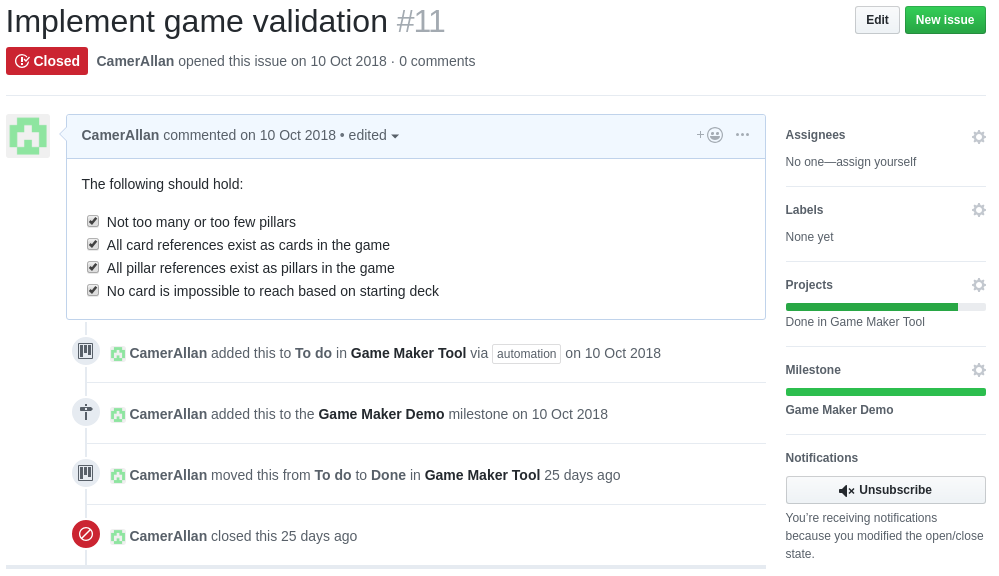
\includegraphics[width=0.9\textwidth]{./images/softeng/issue.png}
	\caption{An example of an issue, note the assigned description, project, and milestone.}
	\label{fig:issue}
\end{figure}

\paragraph{Projects} Issues alone can become unorganised, so I made use of GitHub's projects feature. 
I split my work into four parts - game, game maker, visualisation and backend then made a project for each of these. 
This allowed me to keep issues relating to different parts of the project separate, making it easier to focus on one section at a time.

\begin{figure}[!h]
	\centering
	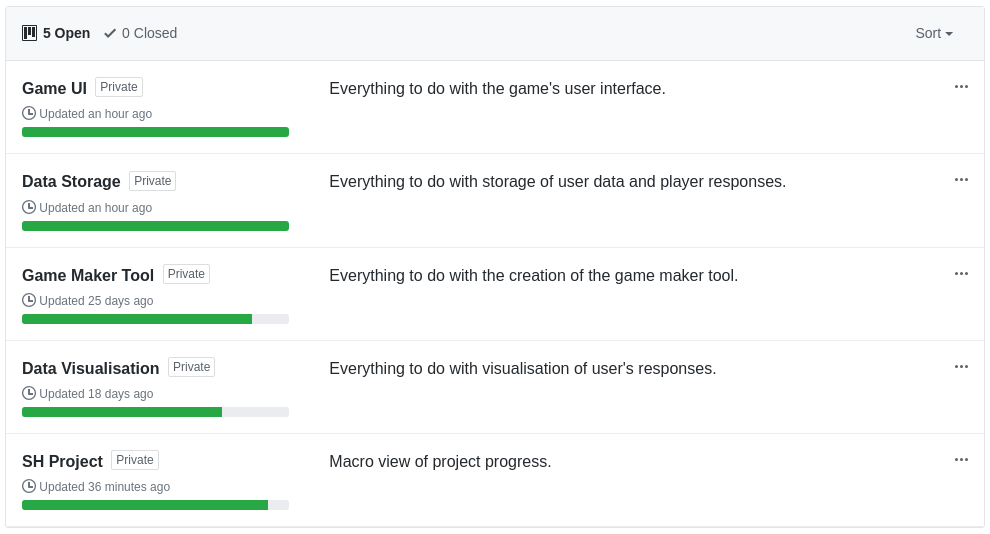
\includegraphics[width=0.9\textwidth]{./images/softeng/projects.png}
	\caption{Project overview page.}
	\label{fig:projects}
\end{figure}

Each project has its own kanban-style~\cite{KBAN} board, used to track its progress, an example of which can be seen in figure~\ref{fig:board}. Issues assigned to a project start in the \c{todo} column. When being worked on, I would move them into \c{In progress}, and finally when closed they are automatically moved to \c{Done}.

The project overview visualises the proportion of issues in each column, providing an instant, accurate depiction of progress.

\begin{figure}[!h]
	\centering
	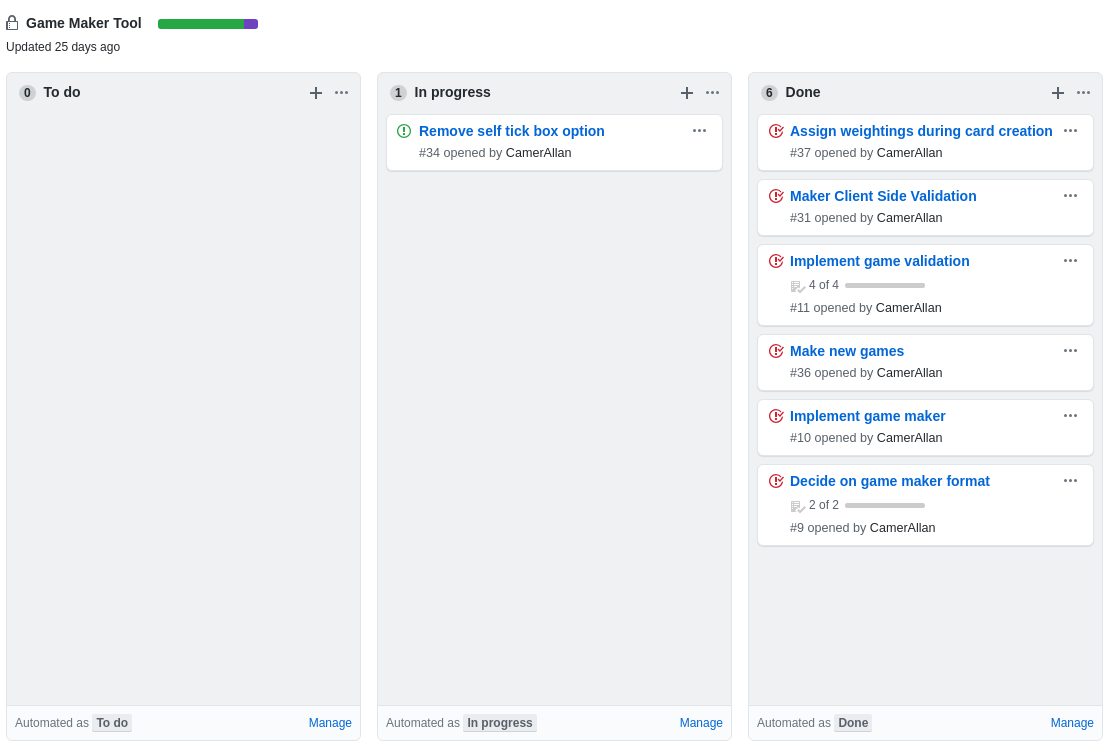
\includegraphics[width=0.9\textwidth]{./images/softeng/board.png}
	\caption{Example project board towards the end of the project.}
	\label{fig:board}
\end{figure}

\paragraph{Milestones} The first step I took in tracking my project was to set my Milestones. These are an aspect of a GitHub project that serve as a deadline, to which issues can be added. 
Completing and closing these issues then automatically provides a visualisation of progress towards a milestone, as can be seen in figures~\ref{fig:closed_milestones} and~\ref{fig:open_milestones}. 
These made for a helpful overview, which was useful both for myself, and for sharing my progress with my supervisor.

I decided on these milestones early on by estimating the dates by which I could complete core parts of the project. As this was done in advance I was not able to be precise with demo dates, however I completed the vast majority of work for each milestone in advance of the deadline, so I consider this a successful element of my planning.

\begin{figure}[!h]
	\centering
	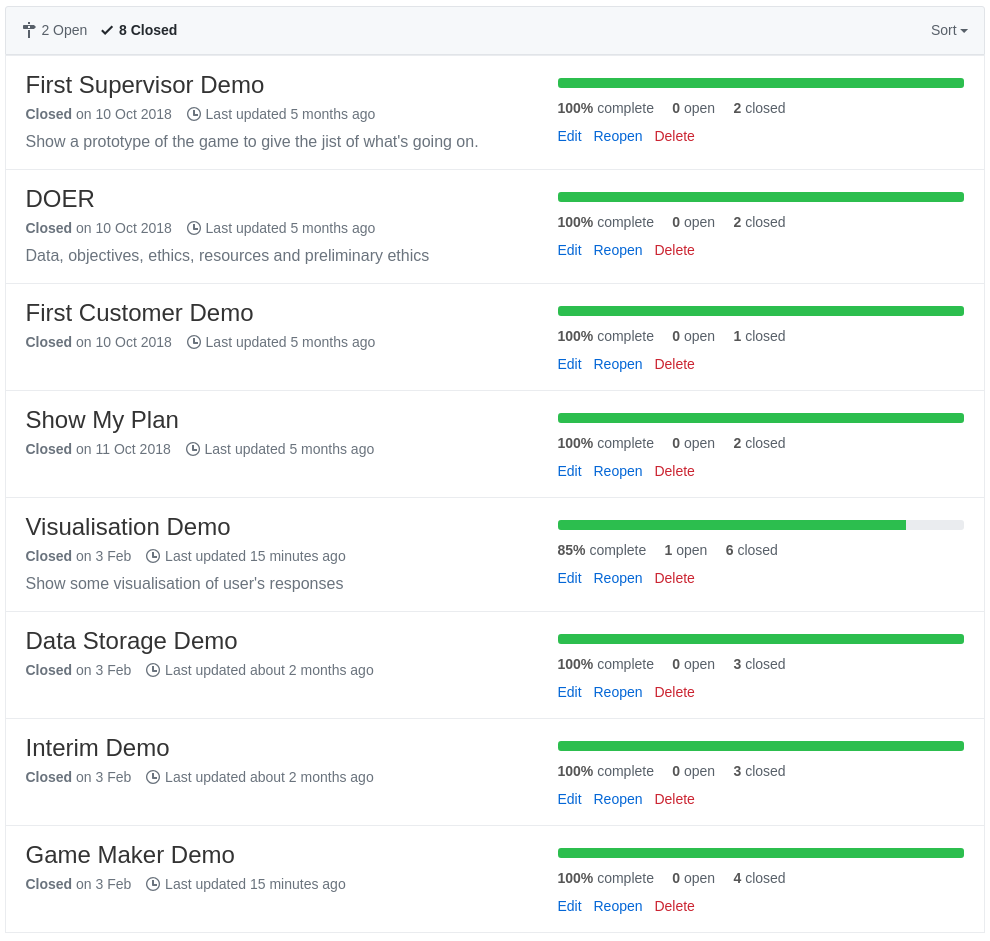
\includegraphics[width=0.9\textwidth]{./images/softeng/closed_milestones.png}
	\caption{Closed (completed) milestones towards the end of the project}
	\label{fig:closed_milestones}
\end{figure}

\begin{figure}[!h]
	\centering
	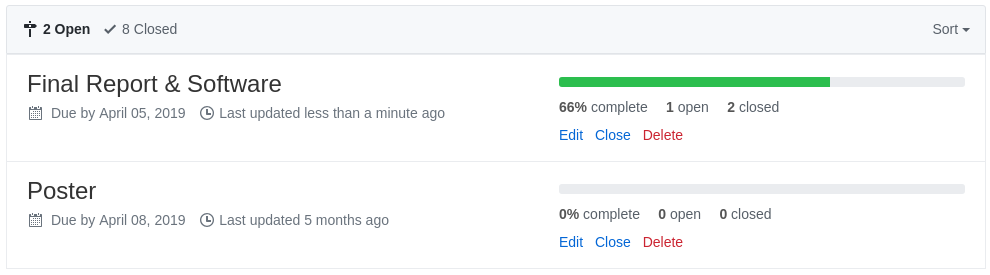
\includegraphics[width=0.9\textwidth]{./images/softeng/open_milestones.png}
	\caption{Open milestones towards the end of the project}
	\label{fig:open_milestones}
\end{figure}


\chapter{Ethics}
All data used for testing and development purposes was fictional. Fictional data was made up by myself, and consists only of user ids. No personal or identifying information was gathered during the user evaluation. Participants' answers were anonymously recorded on paper forms and kept in a secure location. The digitised forms were stored in an encrypted location.
\chapter{Design}

\todo{}

\section{Gameplay Overview}
\todo[inline]{Maybe draw an example as this is a bit confusing}
The game provides a fairly straightforward experience from the user's point of view.
Conceptually, it is a card game, so I will describe it as such.
The game consists of three decks which I dub `in play', `out of play' and `reserve'. In addition to this, there are $n$ `pillars' - these are attributes of importance within the game story's context. Each of these has a minimum, maximum and current value.
The `in play' deck has a defined starting set of cards, with the `reserve deck' containing all others - `out of play' starts empty.
Both decks are shuffled at the start of the game, and each pillar has a predefined starting value.

The player draws and reads a card from the play deck, each one showing the following information:

\begin{itemize}
    \item Title
    \item Description
    \item Choice \#1 (`accept')
    \item Choice \#2 (`reject')
    \item Requirements to draw
\end{itemize}
Each choice on a card consists of text detailing the response, and the effects of the response. Effects are made up of two parts - pillar changes, and cards added/removed. Pillar changes specify amounts to add or remove from one or more pillars. Cards added/removed defines which cards should be moved between `out of play' and `reserve'.
Requirements to draw consists of conditions that the current pillar levels must satisfy in order for this card to be drawn.

After each choice made (turn), any cards in `out of play' the meet the current pillar requirements are moved to `in play', and any `in play' that do not are moved to `out of play'. 

The game ends when any of the pillars fall to their minimum value.

\section{UI}

\subsection{Game}
As described above, the game sounds like a lot of effort on behalf of the player, having to sort and shuffle cards. Fortunately, this effort can be removed completely through work done by the computer. This leaves a simple game from the user perspective; users are presented with a card, make a choice, and get the next card.

This meant that the design for the game UI could also be simple. Figure \ref{fig:game_comp} shows my first design for this UI alongside the final product. Initially, I wasn't sure whether the pillars should be visible to the user, however after some testing it was clear that they were needed to provide the player with feedback as they played the game, so they were later added to the top of the screen.

\begin{figure}[!h]
	\centering
	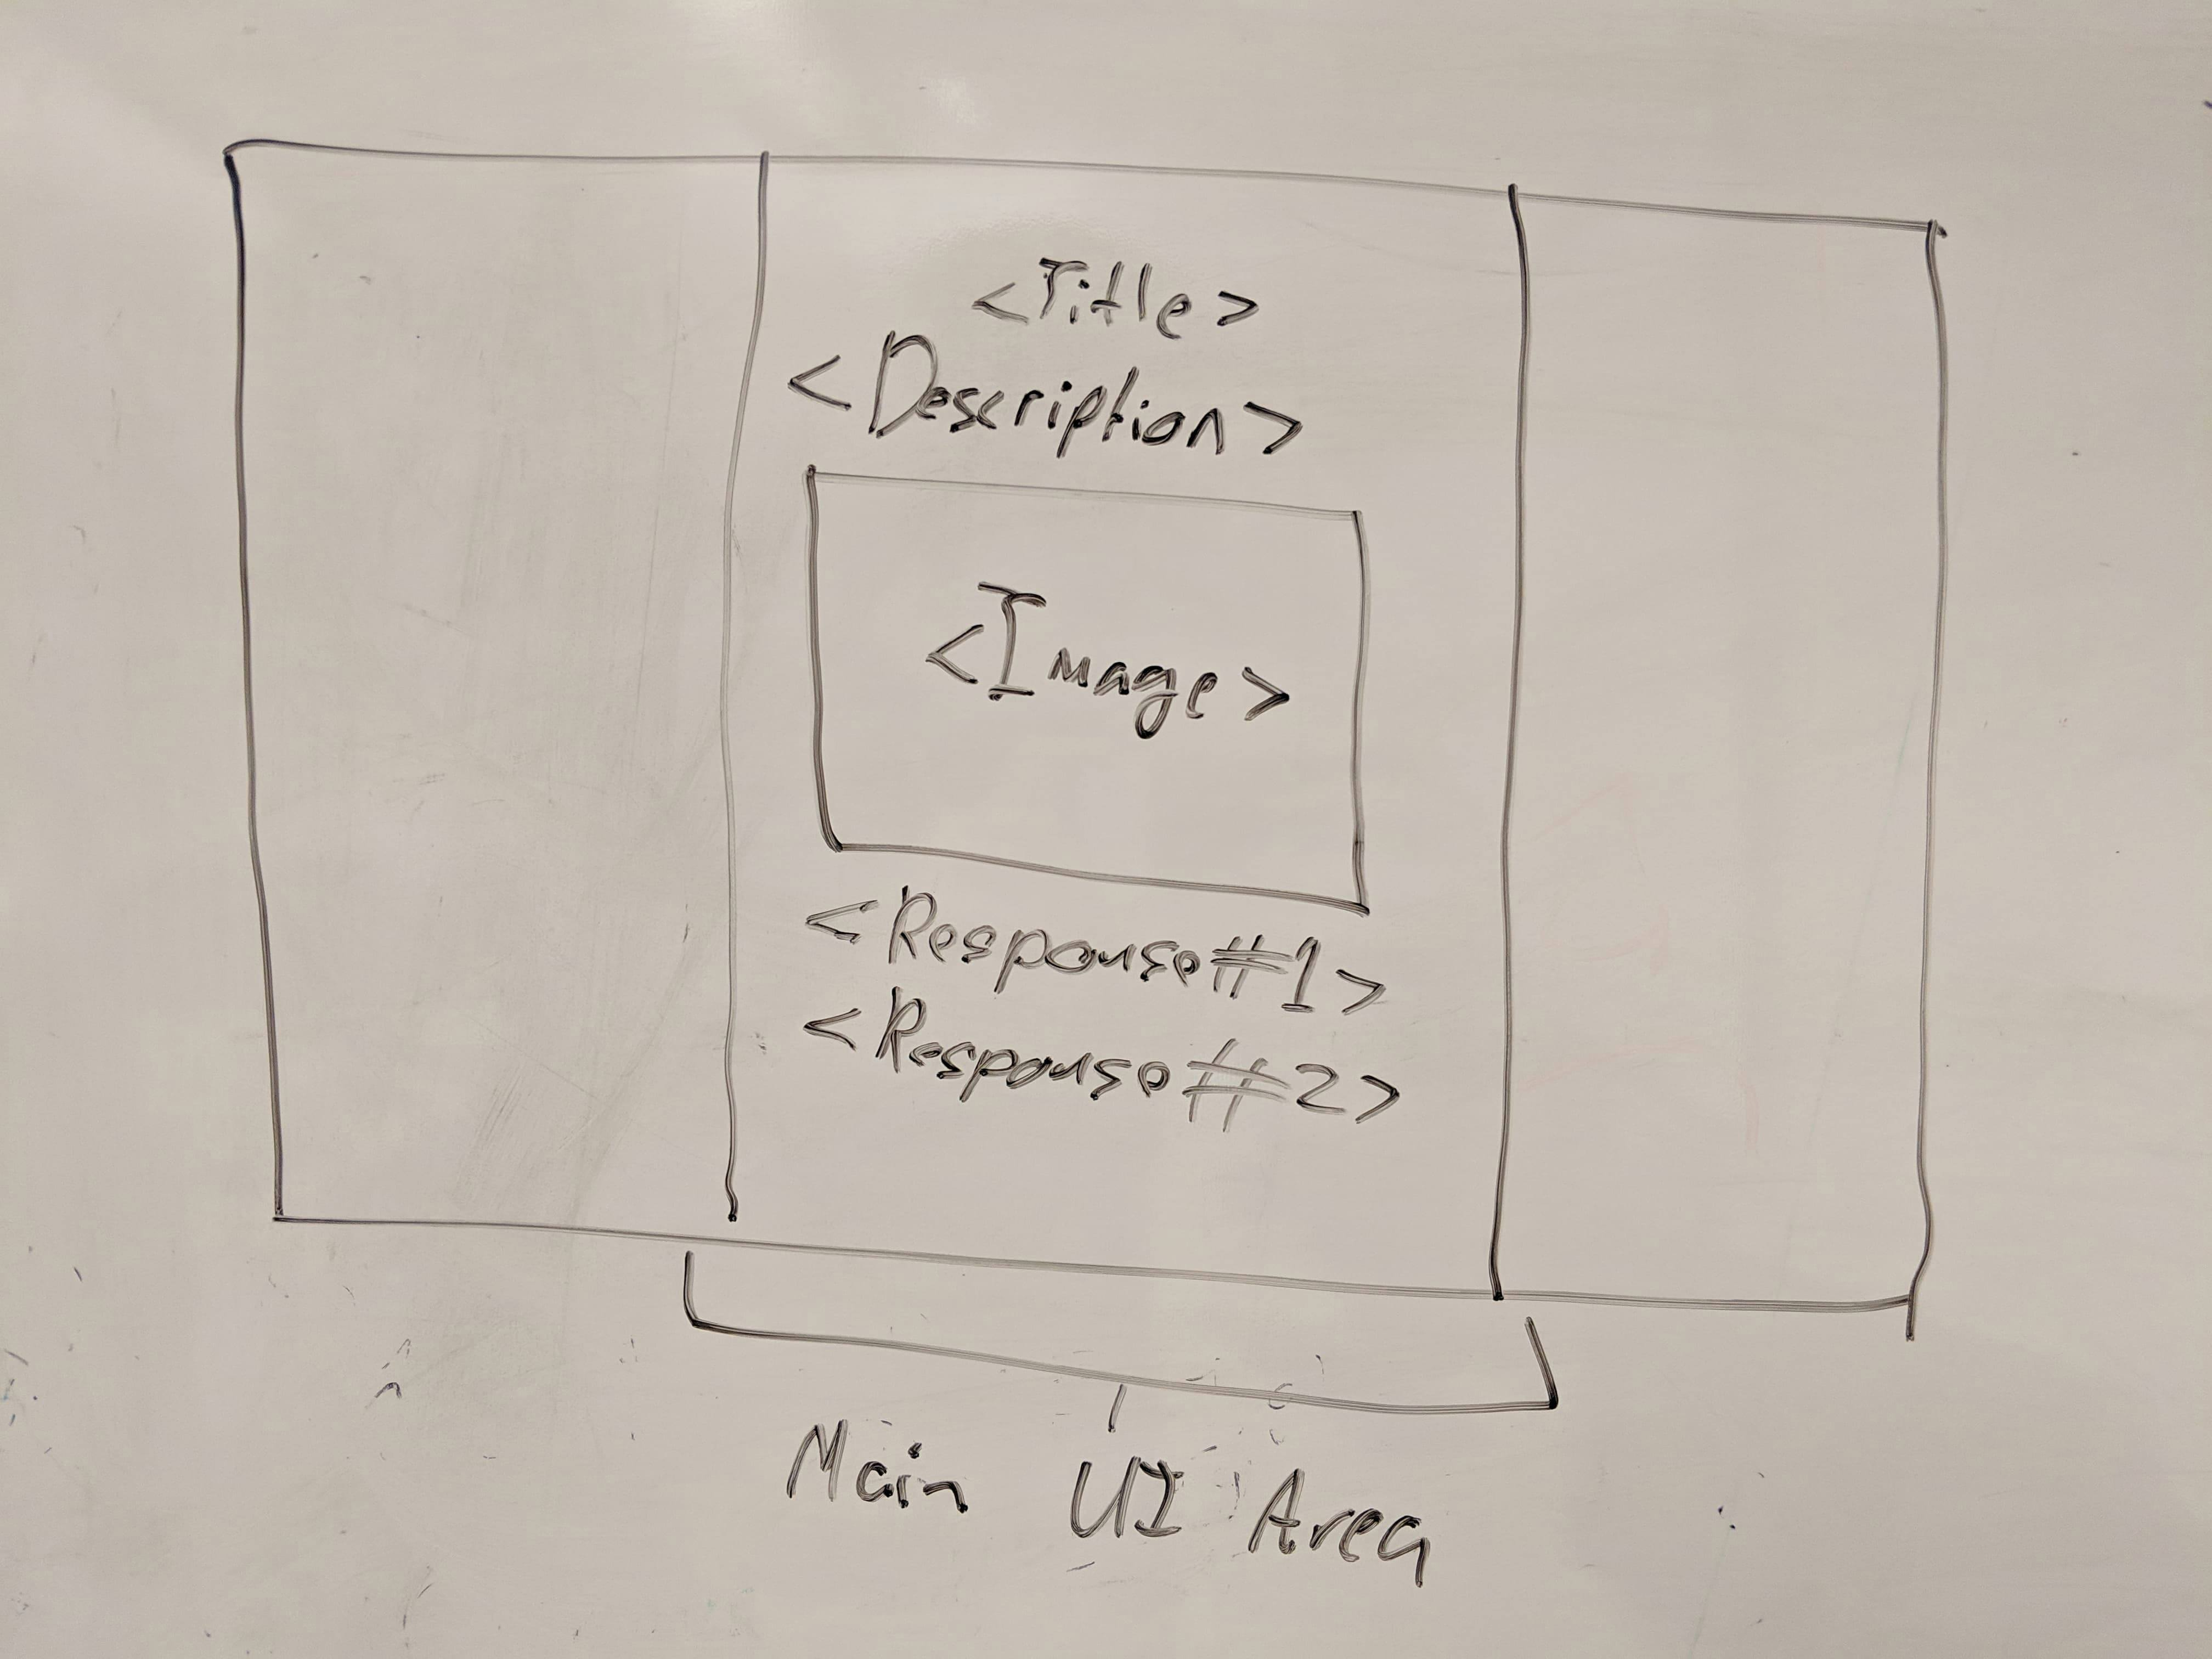
\includegraphics[width=0.36\textwidth]{./images/design/game_drawing.jpg}
	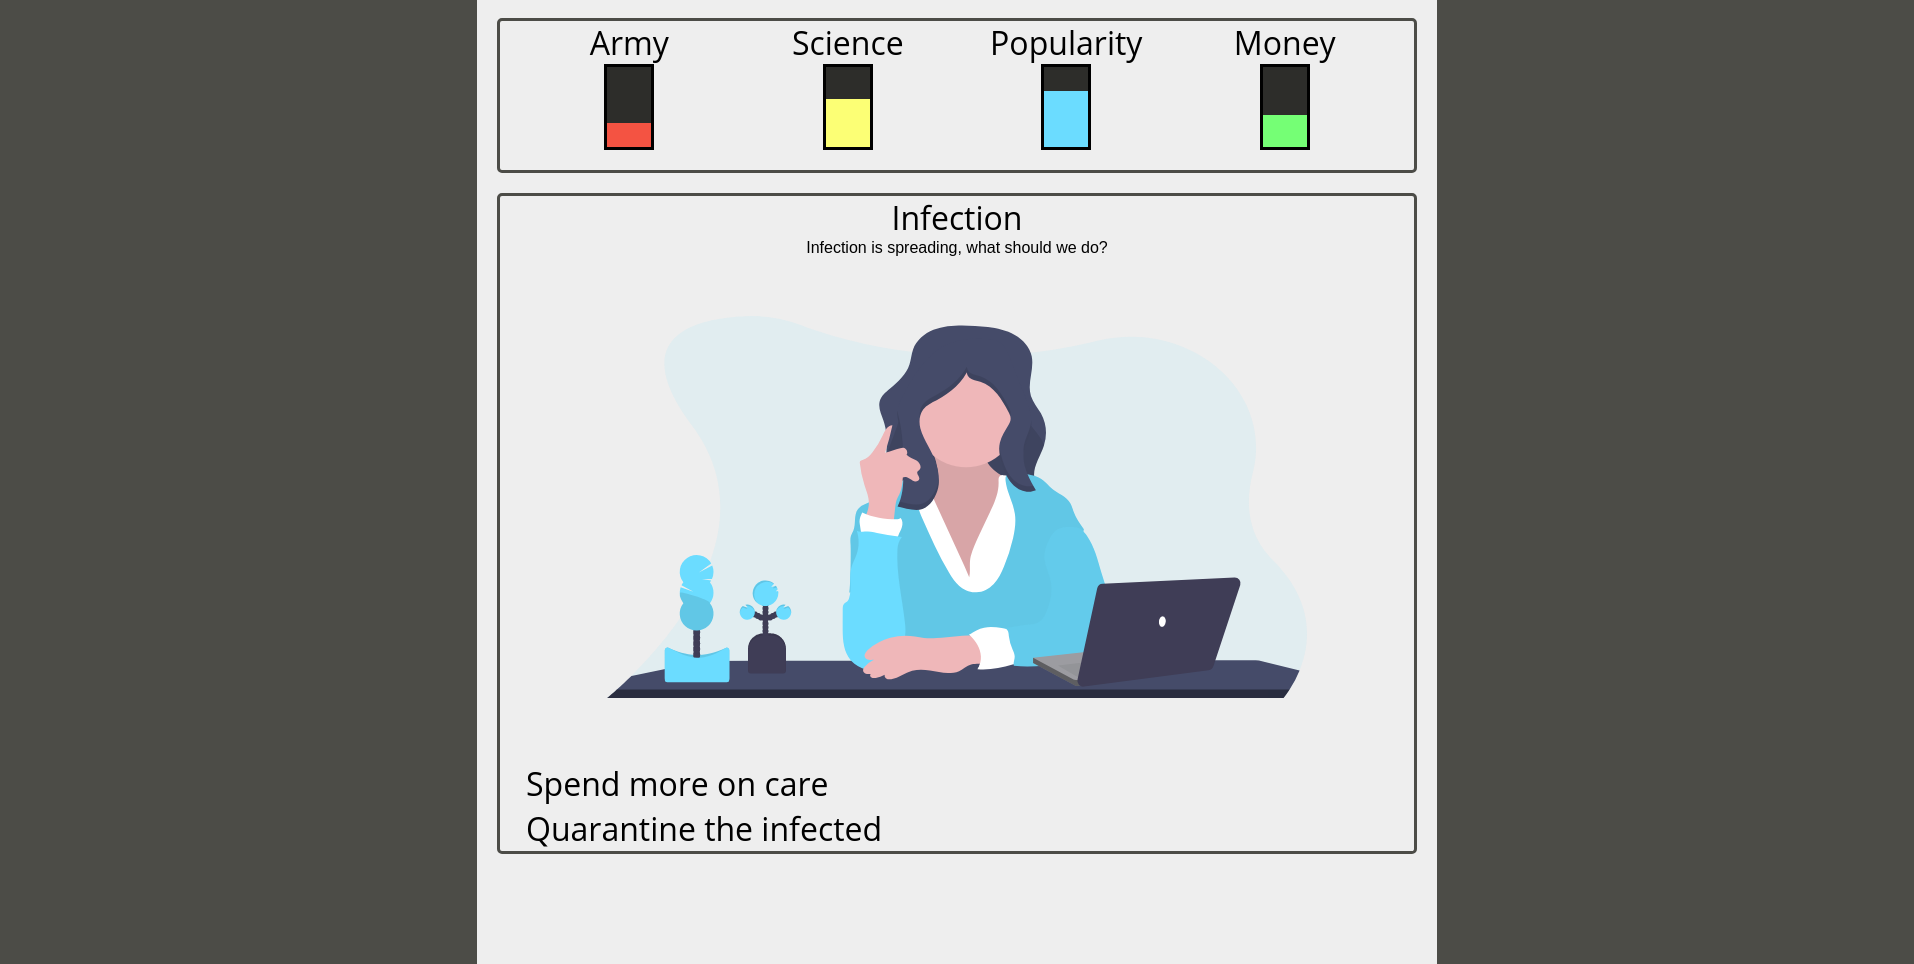
\includegraphics[width=0.54\textwidth]{./images/design/game.png}
	\caption{Comparison between initial and final designs for the game UI}
	\label{fig:game_comp}
\end{figure}

Pillars are displayed as vertical bars at the top of the screen, each having their own fill colour (customisable through game definition). I was inspired to add this colour customisation by other survey gamification tools, as a way to make the game more visually engaging, without forcing a colour scheme that could conflict with the desires of admin users. Pillars fill from bottom to top, and represent where the current value lies between the defined min and max.

\begin{figure}[!h]
	\centering
	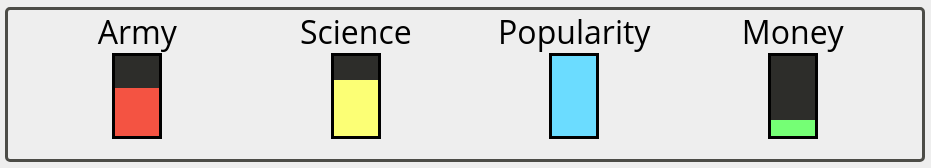
\includegraphics[width=0.9\textwidth]{./images/design/pillars.png}
	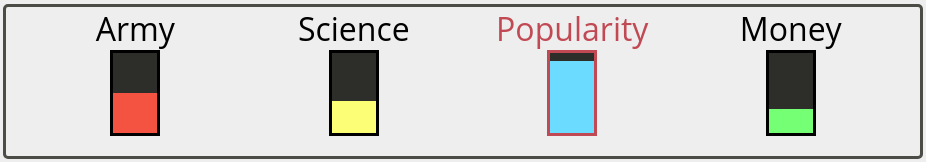
\includegraphics[width=0.9\textwidth]{./images/design/hover.png}
	\caption{Visualisation of a negative outcome; the red outline around \c{Popularity} }
	\label{fig:colour_comp}
\end{figure}

The image shown with a given card is dependent upon the pillars the card influences, as seen in figure \ref{fig:advisor_comp}. In this example game, I gave each pillar an `advisor' image, so that the advisor representing the pillar most affected by a card is shown.

\begin{figure}[!h]
	\centering
	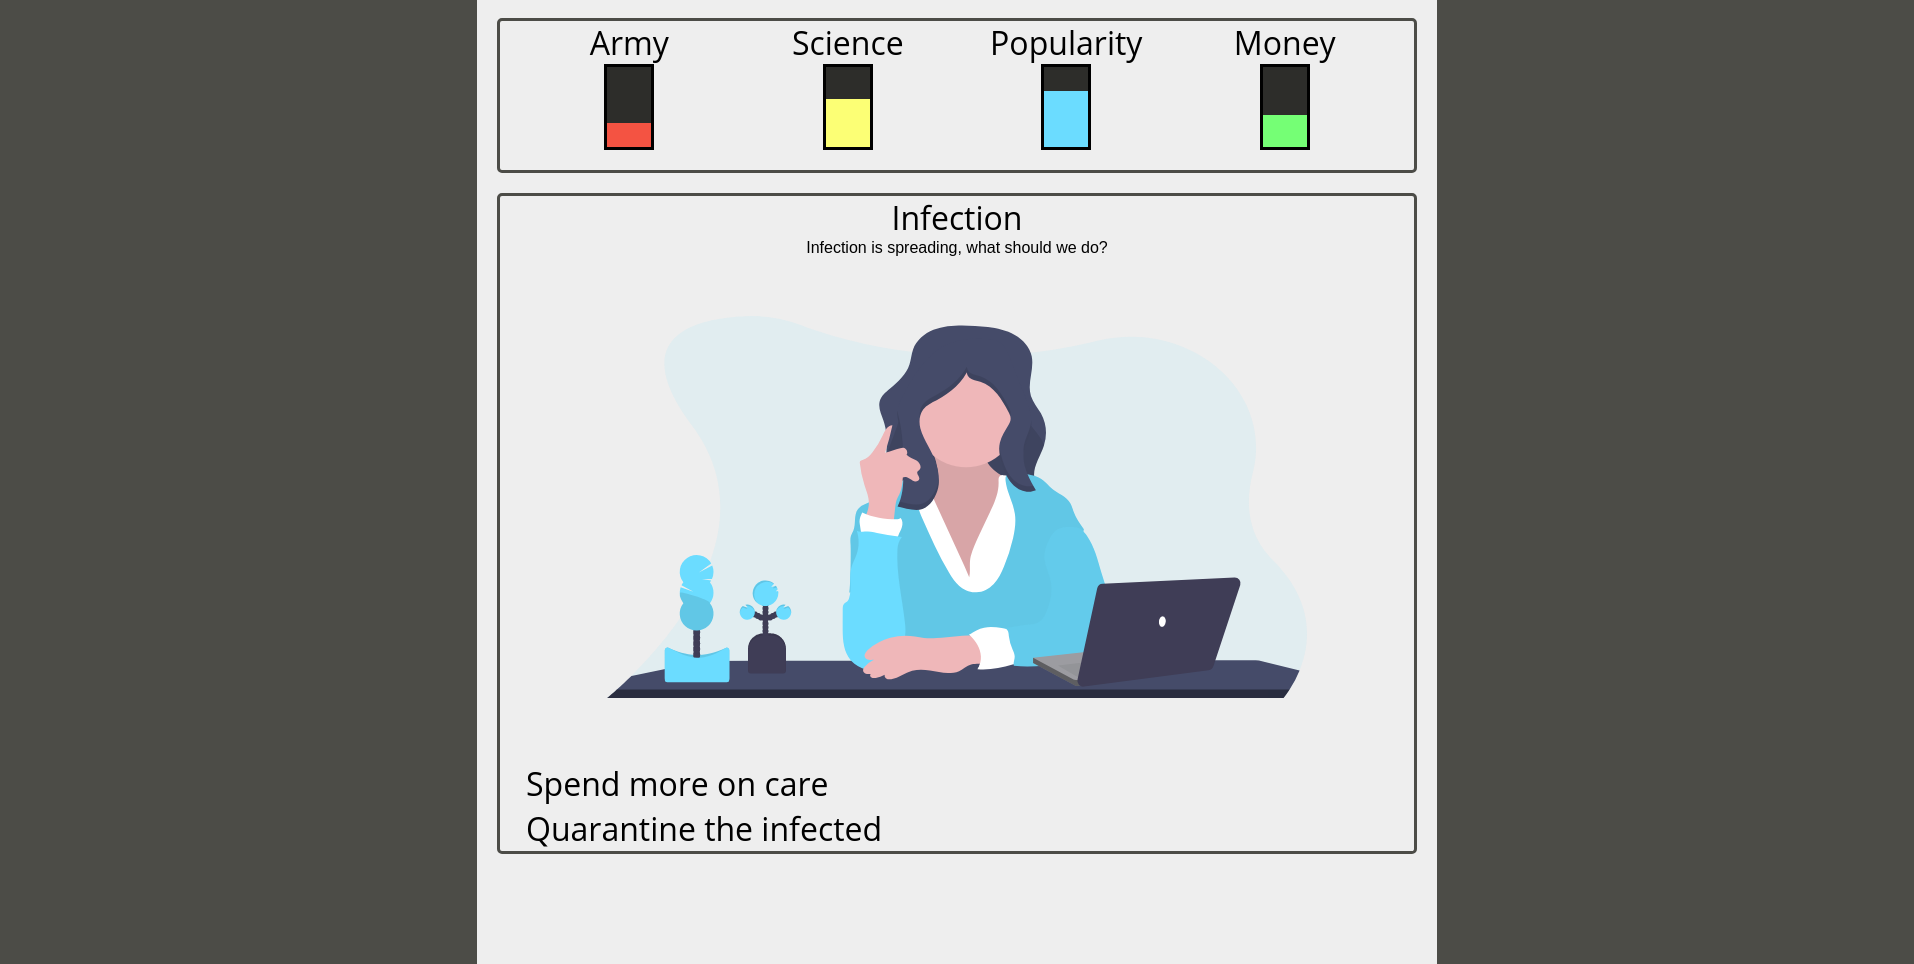
\includegraphics[width=0.45\textwidth]{./images/design/game.png}
	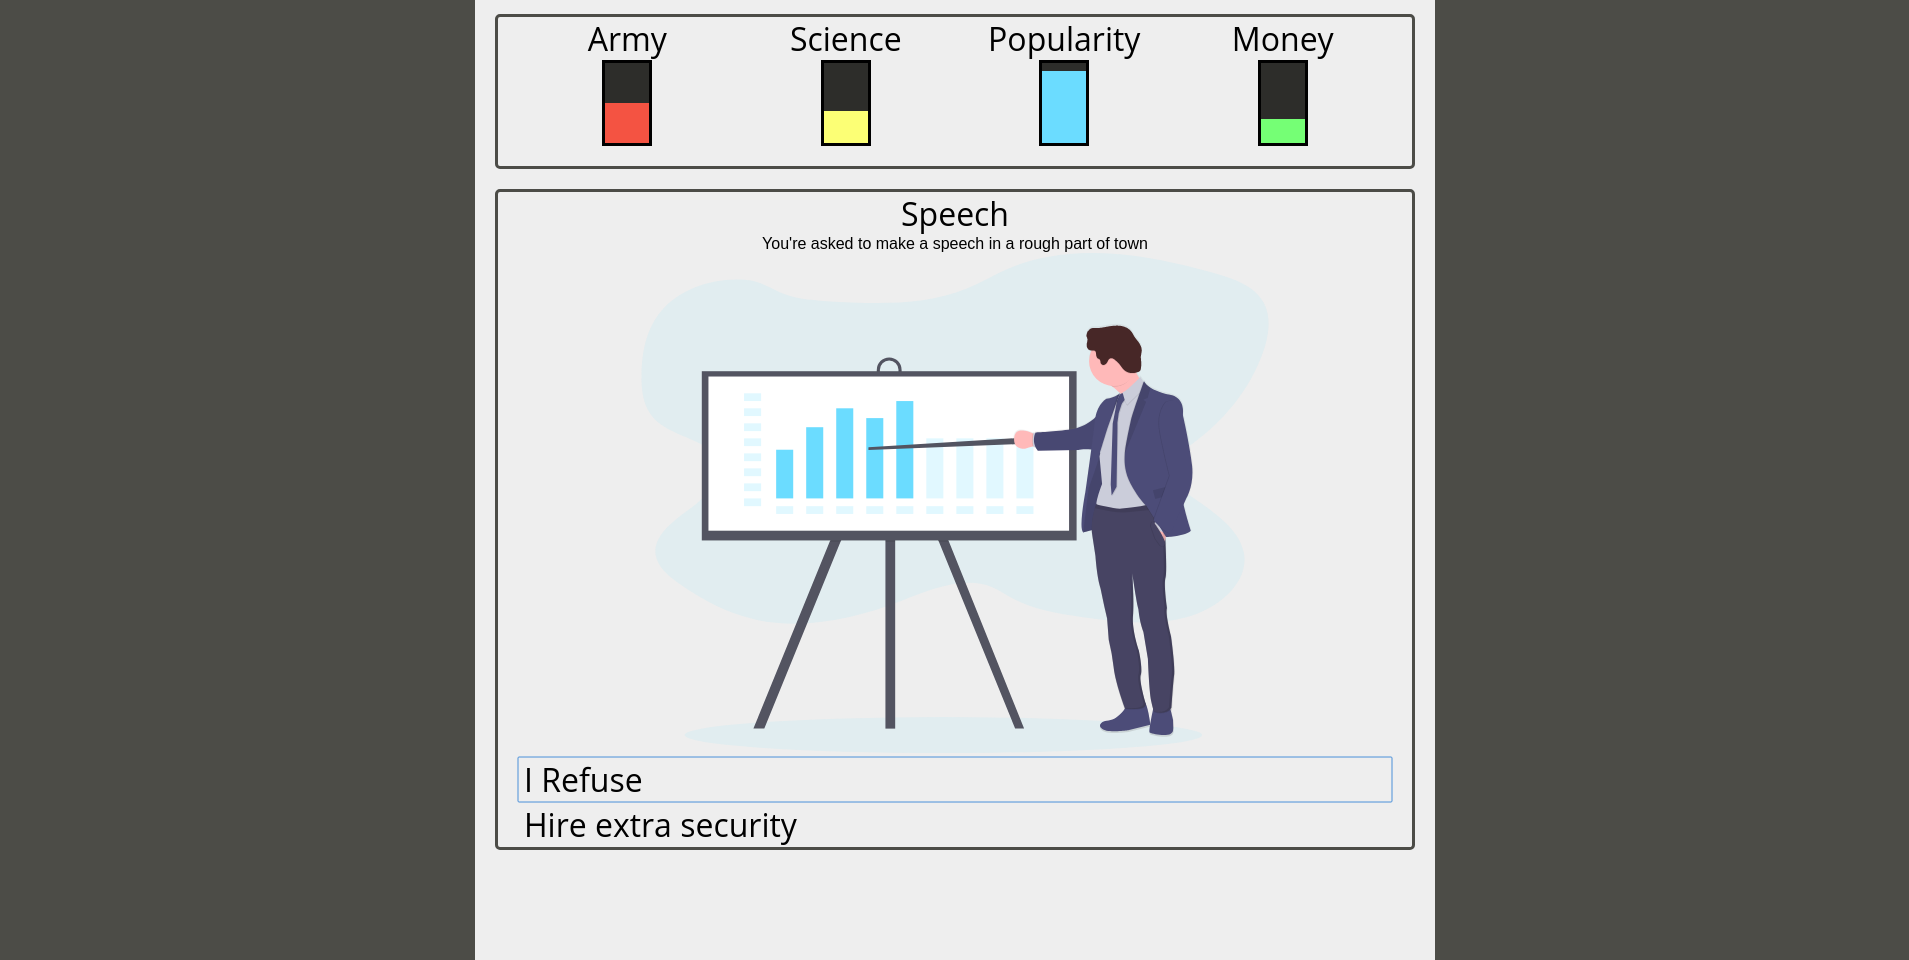
\includegraphics[width=0.45\textwidth]{./images/design/ecman_blue.png}
	\caption{These cards primarily affect different pillars, so they have different associated images}
	\label{fig:advisor_comp}
\end{figure}

As seen in figure \ref{fig:colour_comp}, not only can the image change, but the primary colour of the image may also change. I decided to include this feature as cards may affect more than one pillar, and this was not being represented when only using different images. With this colour shifting implemented, the image can represent secondary pillar effects.

\begin{figure}[!h]
	\centering
	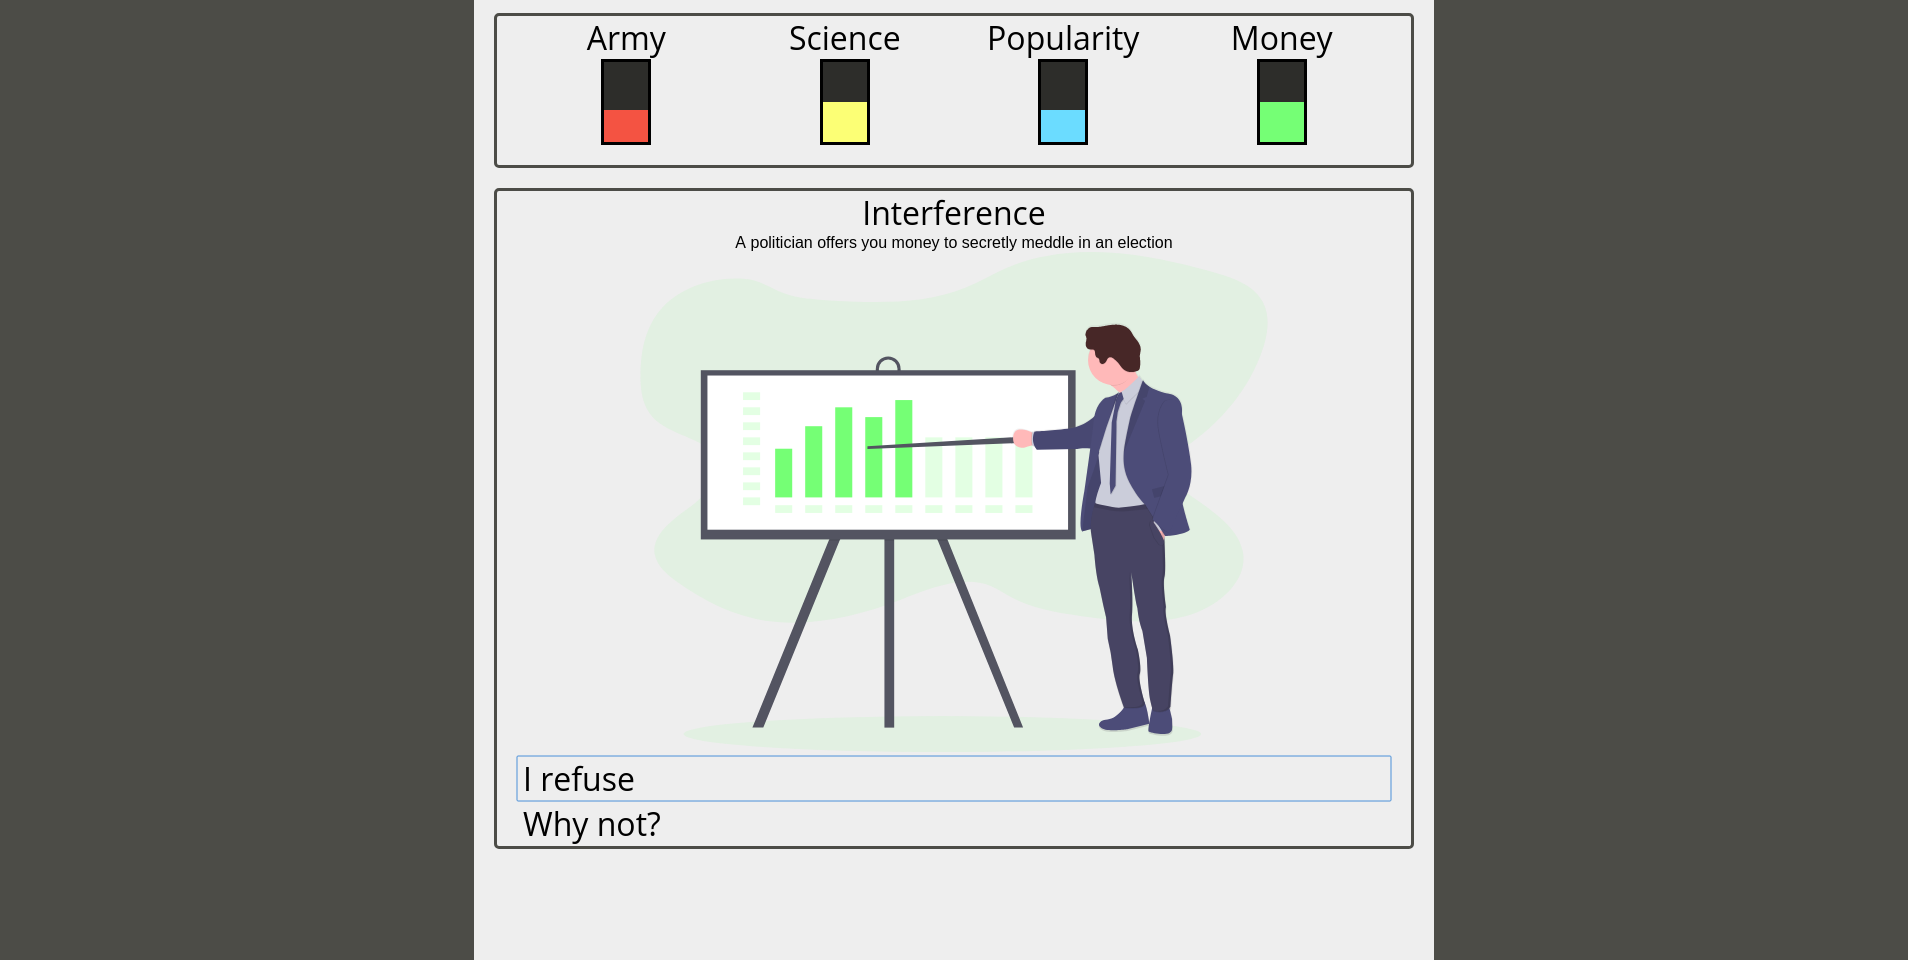
\includegraphics[width=0.45\textwidth]{./images/design/ecman_green.png}
	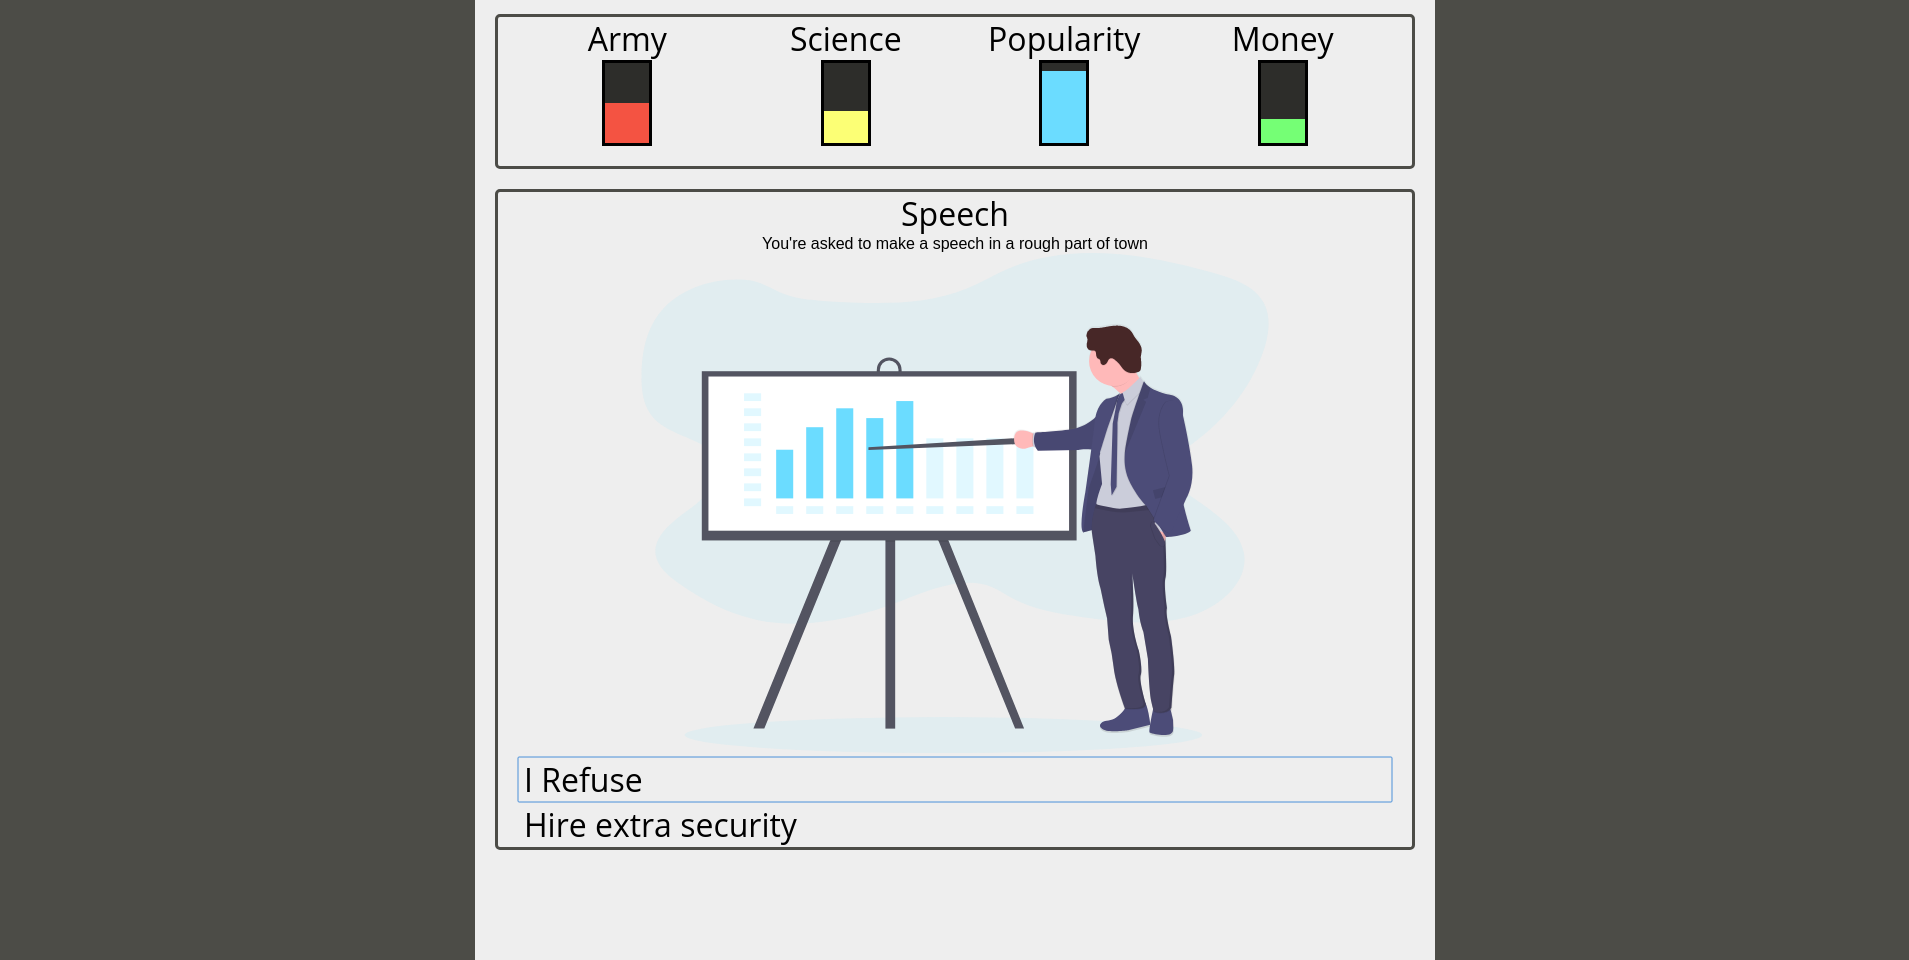
\includegraphics[width=0.45\textwidth]{./images/design/ecman_blue.png}
	\caption{Both of these cards primarily affect the \c{Money} pillar (they are being presented by the \c{Money} advisor) however the second also affects \c{Popularity}, so has a blue primary colour}
	\label{fig:colour_comp}
\end{figure}

\subsection{Admin tools}

\subsubsection{Game Maker}
The game maker interface was the most challenging to design, as I wanted the user to be able to maintain a high-level overview of the game while adding and editing pillars and cards. 
After thinking this through, I initially settled on the design depicted in figure \ref{fig:game_maker}. The main theme is that editing is done in the left panel, while the right side continues to show an interactive view of the game, including a visualisation of the relationships between cards.
The final design ended up being roughly the same, however the card view is not as complex - connections between cards are not visualised, as after more consideration of the relationships involved, I could not think of a clear way to show this.
The cards are instead displayed in a grid in the final design.

\begin{figure}[!h]
	\centering
	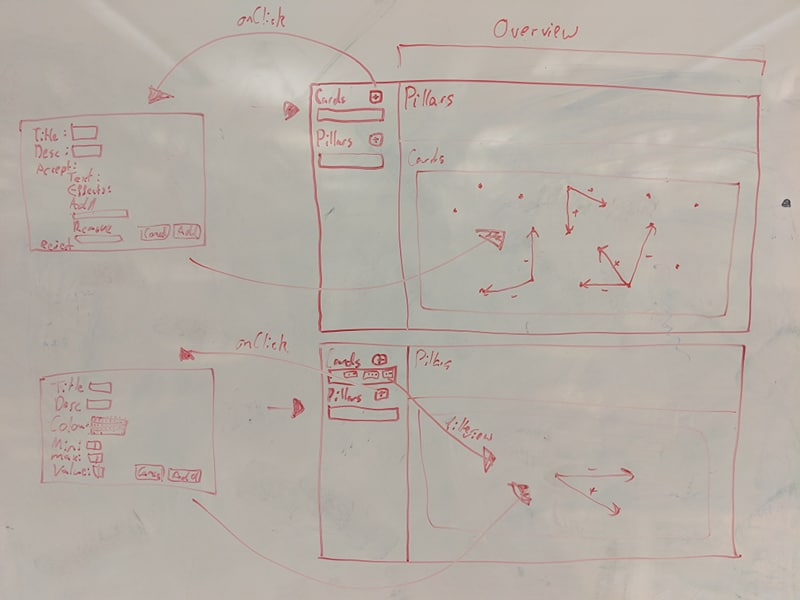
\includegraphics[width=0.36\textwidth]{./images/design/game_maker_drawing.png}
	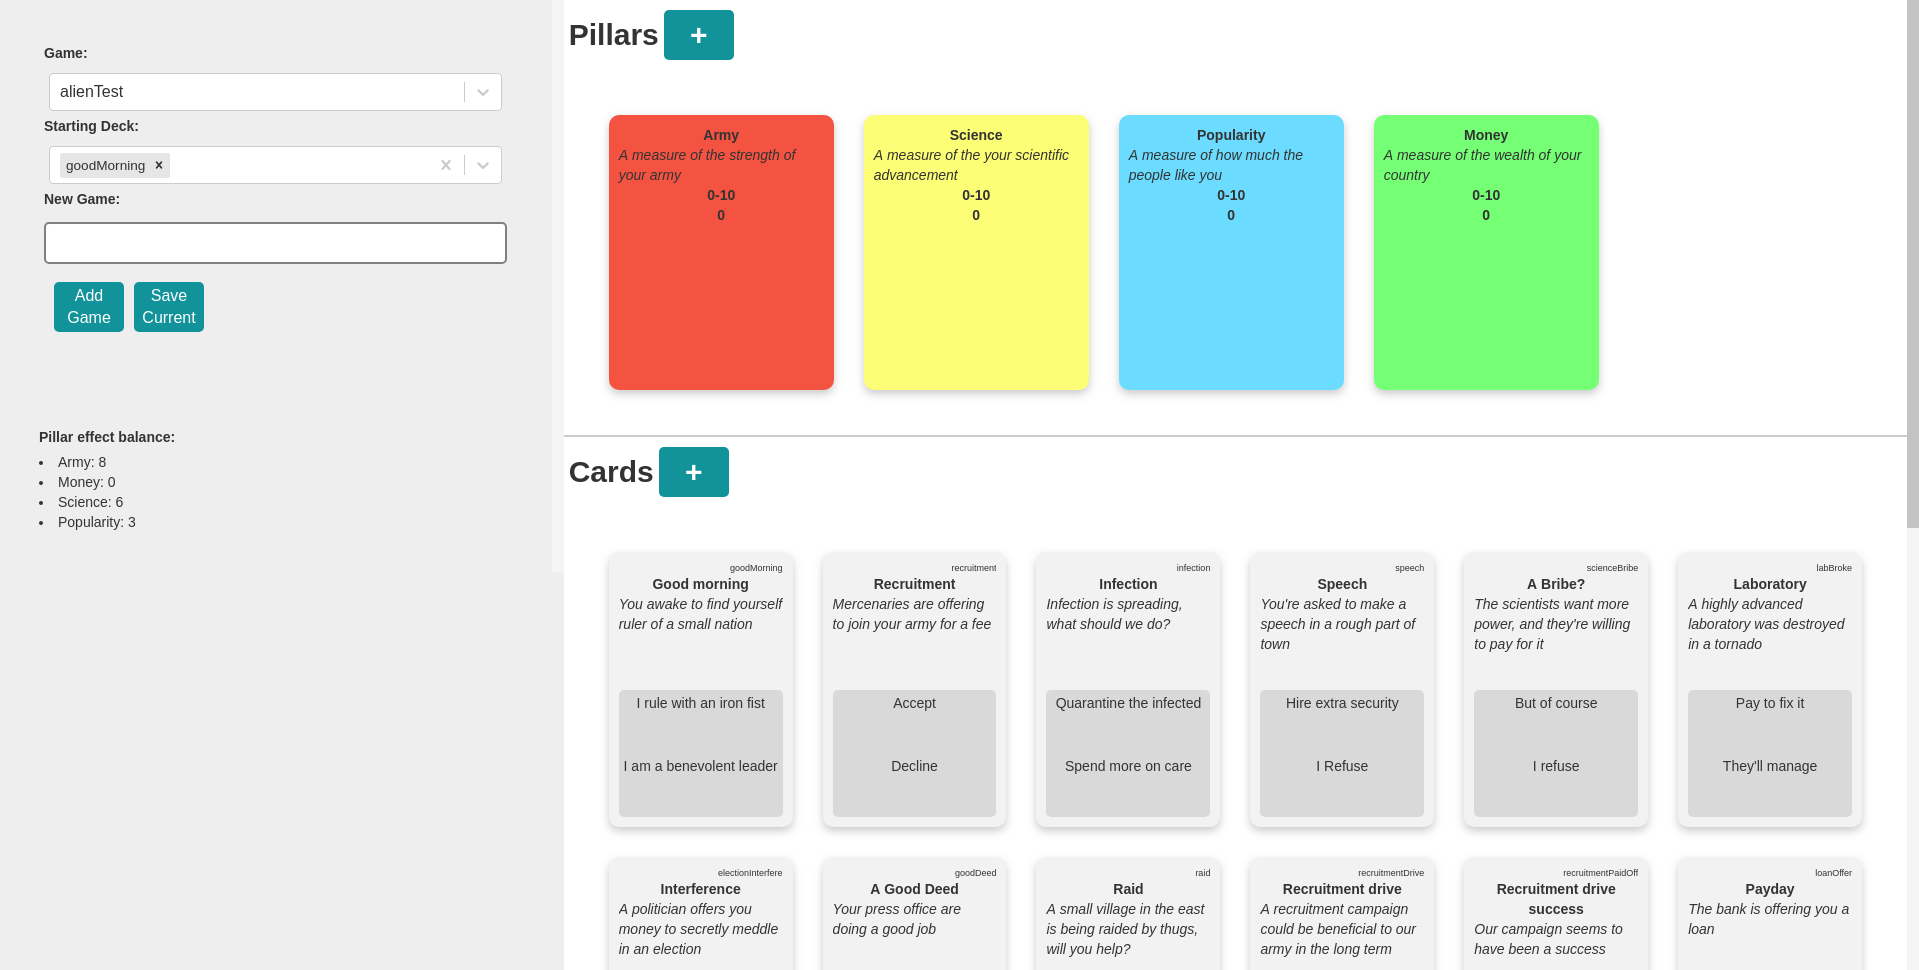
\includegraphics[width=0.54\textwidth]{./images/design/game_maker.png}
	\caption{Comparison between initial and final designs for the game maker. Shown is the example game I created for demonstration purposes.}
	\label{fig:game_maker}
\end{figure}

In the section on the right, the user can see the game pillars and cards that they have created. This side is scrollable, while the left section remains in view. If the details of a card are too large for the view, the text fades out. The card view can be expanded by hovering over it, as seen in figure \ref{fig:expand} - when this is done, other cards shrink and move to allow the extra space. New cards and pillars can be added with the large \c{+} buttons by the headers, while existing ones can be edited by clicking on them. Both of these options opens the edit view on the left section.

\begin{figure}[!h]
	\centering
	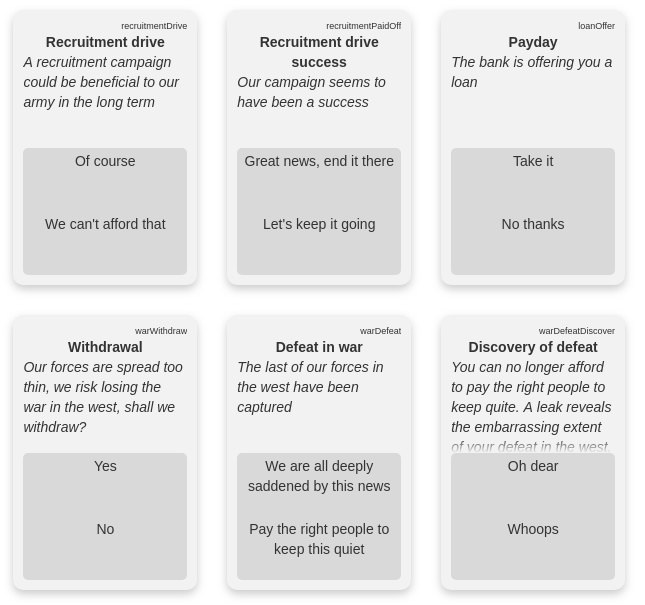
\includegraphics[width=0.45\textwidth]{./images/design/cards_not_expanded.png}
	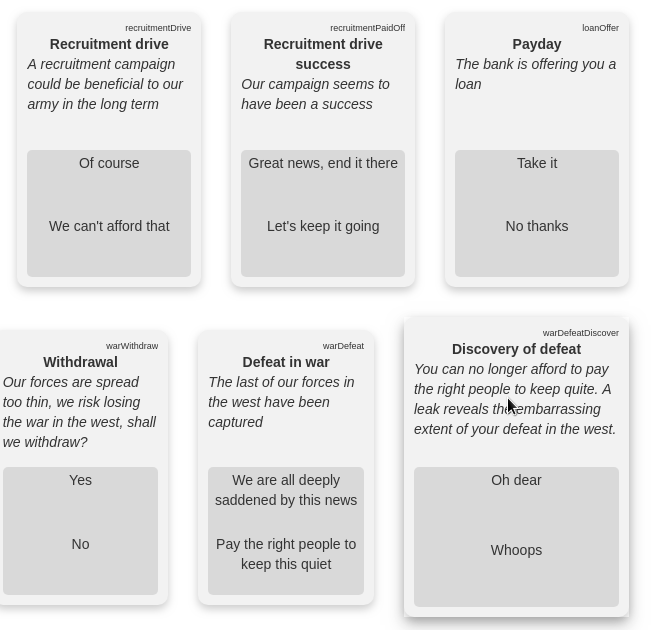
\includegraphics[width=0.45\textwidth]{./images/design/cards_expanded.png}
	\caption{Demonstration of hover expanded view (note that the full text is cut off on the left, readable on the right)}
	\label{fig:expand}
\end{figure}

The left section provides contextual menus. When no pillar or card is selected, it provides high-level functionality, such as saving, switching, or creating new game definitions. Also present here is starting deck selection, game balance information and any warnings.

The pillar effect balance provides the admin user with an idea of how balanced their game is in its current state. This is done by summing all of the effects that are applied to each pillar for any given response to all cards. This acts as an indicator of how well a user is likely to do if they randomly pick their responses. The higher the balance values, easier the game.

Warnings appear when a card has no chance of being added to the game. This means that a card has been created, but it is neither in the starting deck, nor is it added by any other card. This is only a shallow check - if card A is added by another card B, which itself is never added, the warning will only appear for card B. I consider this acceptable, as once card B is added or deleted, the situation will be resolved.

\begin{figure}[!h]
	\centering
	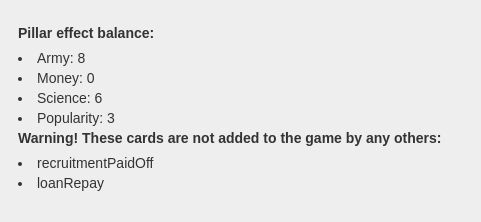
\includegraphics[width=0.6\textwidth]{./images/design/info.png}
	\caption{Info on left panel. Note the two warnings, which appeared on removing \c{recruitmentPaidOff} and \c{loanRepay} from all `cards added' lists}
	\label{fig:info}
\end{figure}

When editing a card, a live preview can be seen at the bottom of the panel, along with buttons to cancel changes, delete, or submit the card. When editing the consequences, adding and removing cards is done through a dropdown list, which allows multiple cards to be selected.

\begin{figure}[!h]
	\centering
	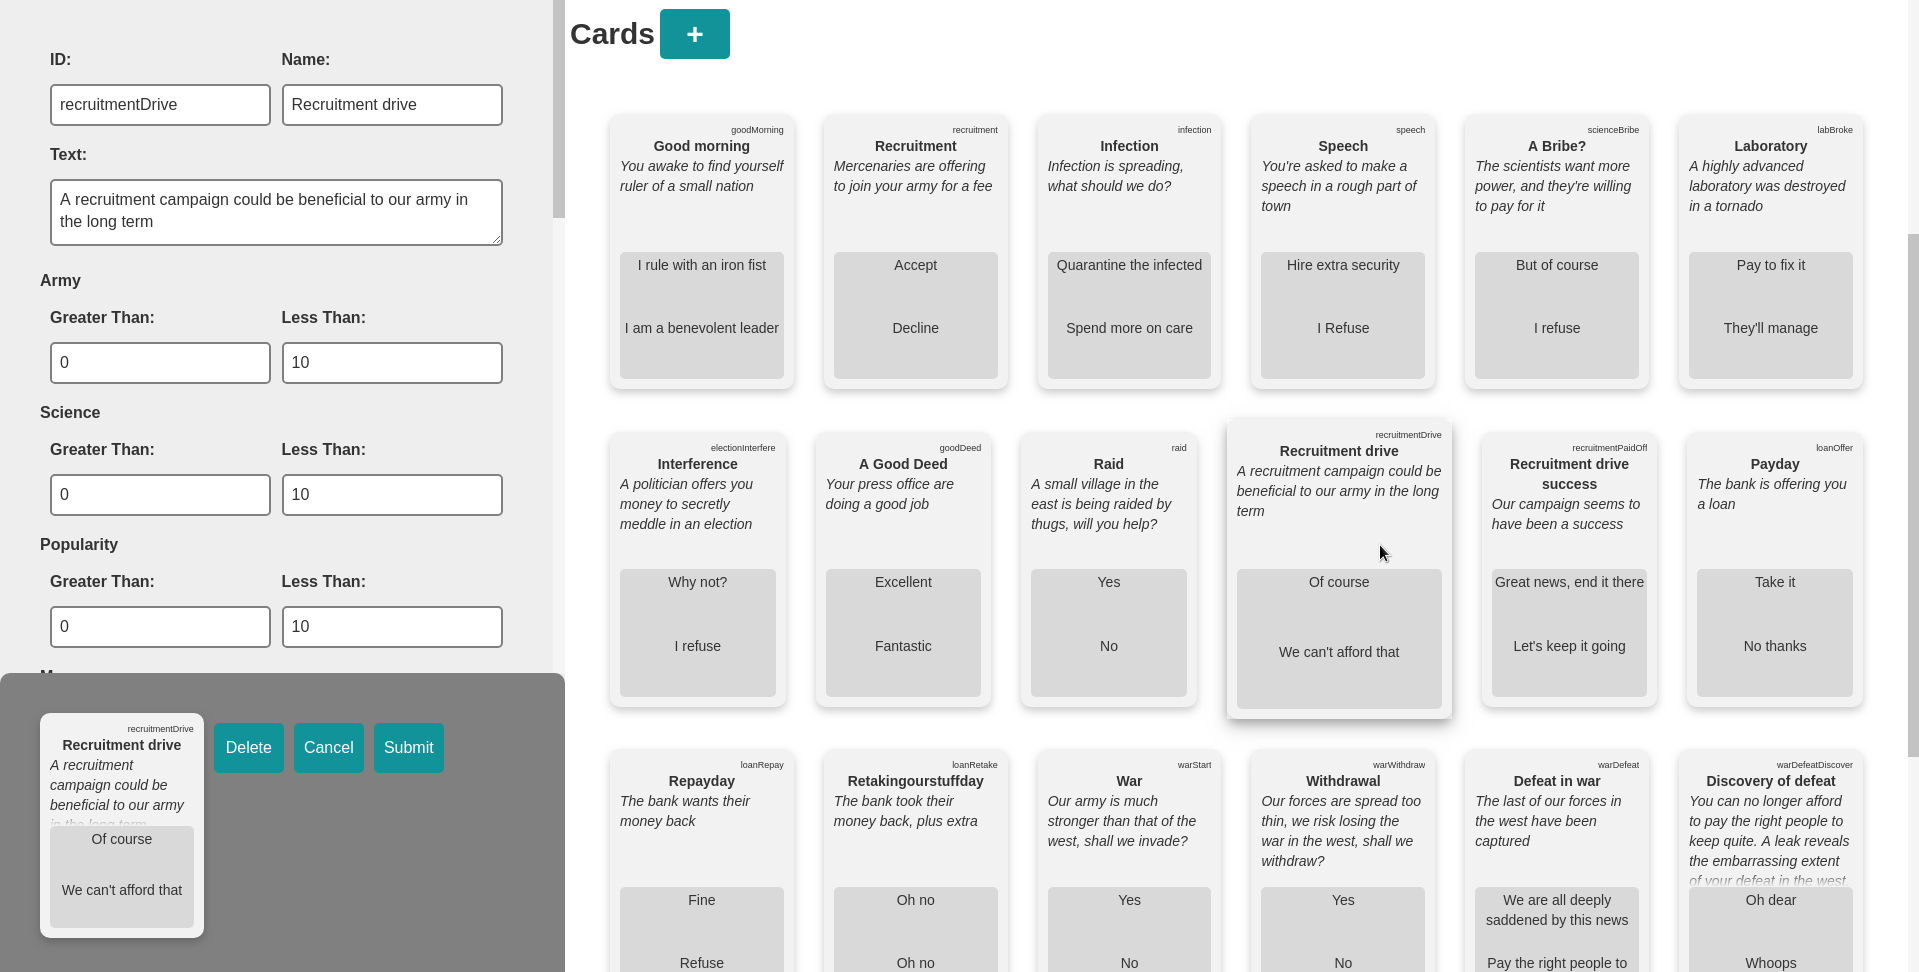
\includegraphics[width=1.0\textwidth]{./images/design/card_edit.png}
	\caption{Card editing view, reached by selecting a card by clicking it.}
	\label{fig:card_edit}
\end{figure}

\begin{figure}[!h]
	\centering
	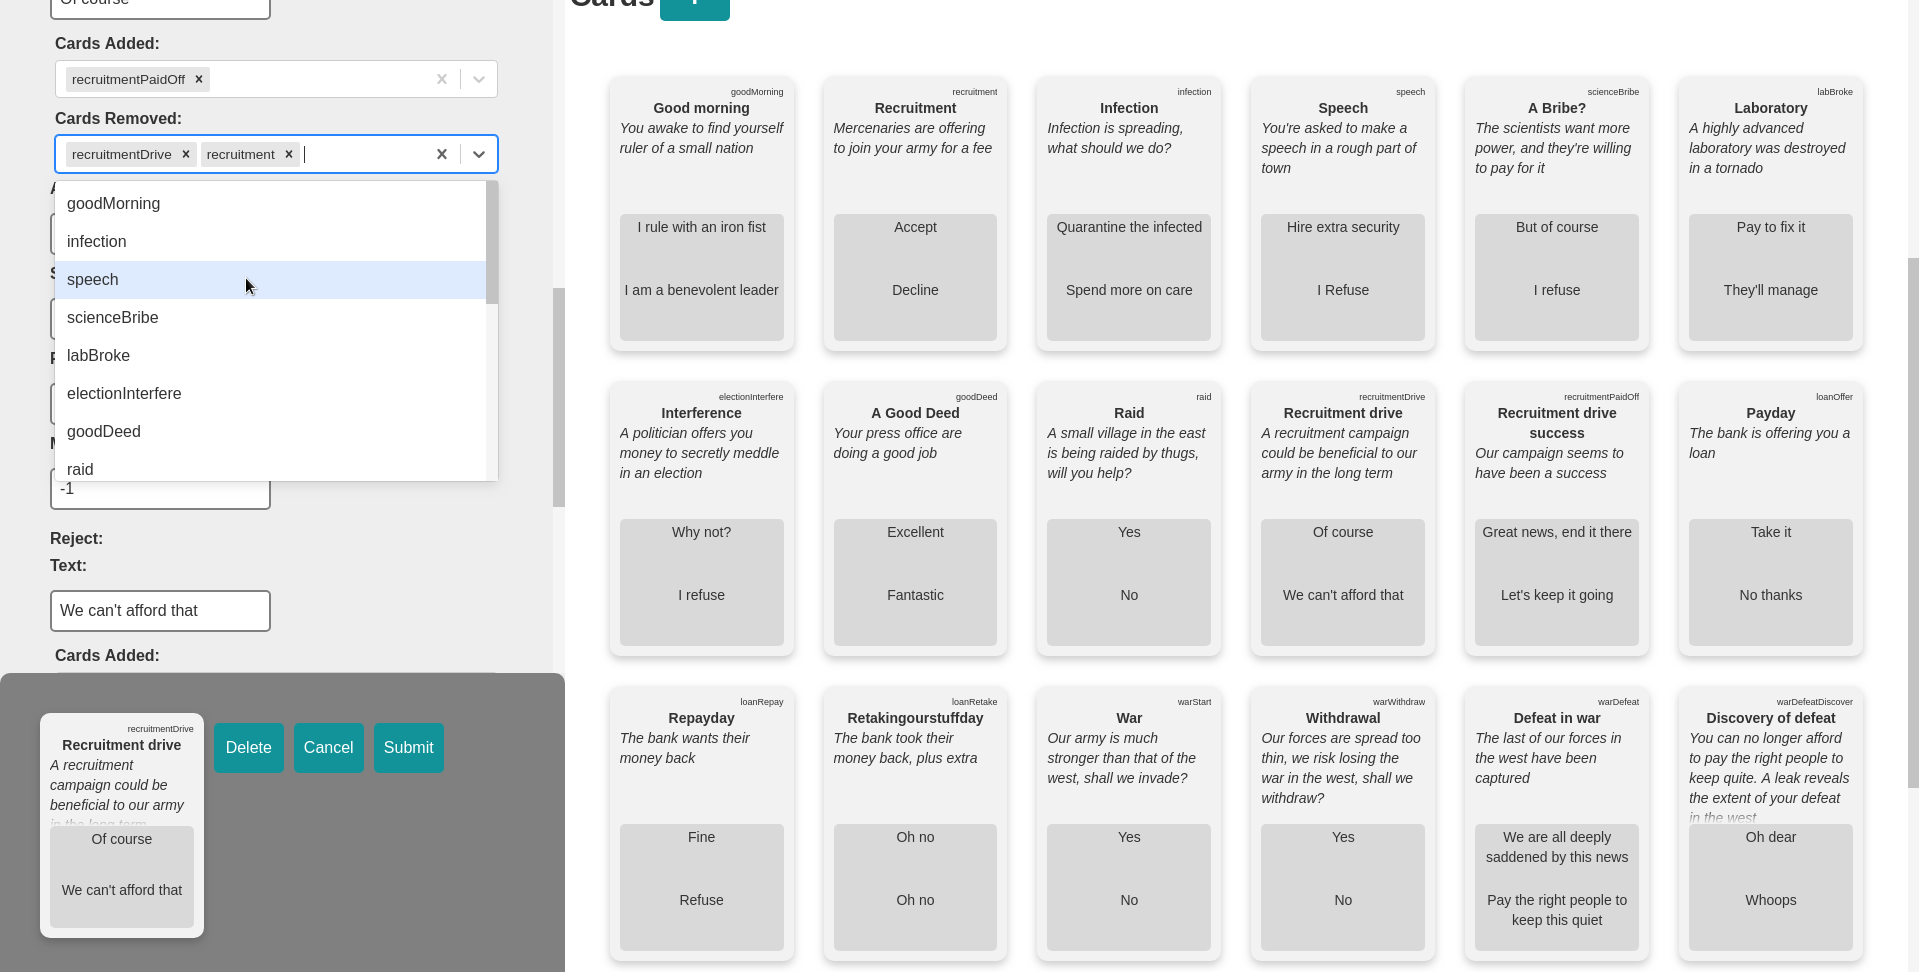
\includegraphics[width=1.0\textwidth]{./images/design/add_card.png}
	\caption{Dropdown showing all other cards that can be added or removed}
	\label{fig:add_card}
\end{figure}

Figure \ref{fig:pillar_edit} shows the pillar editing menu, which is very similar to the card editing view. The colour of the pillar can be entered as a hex value, which is immediately reflected in the preview below.

\begin{figure}[!h]
	\centering
	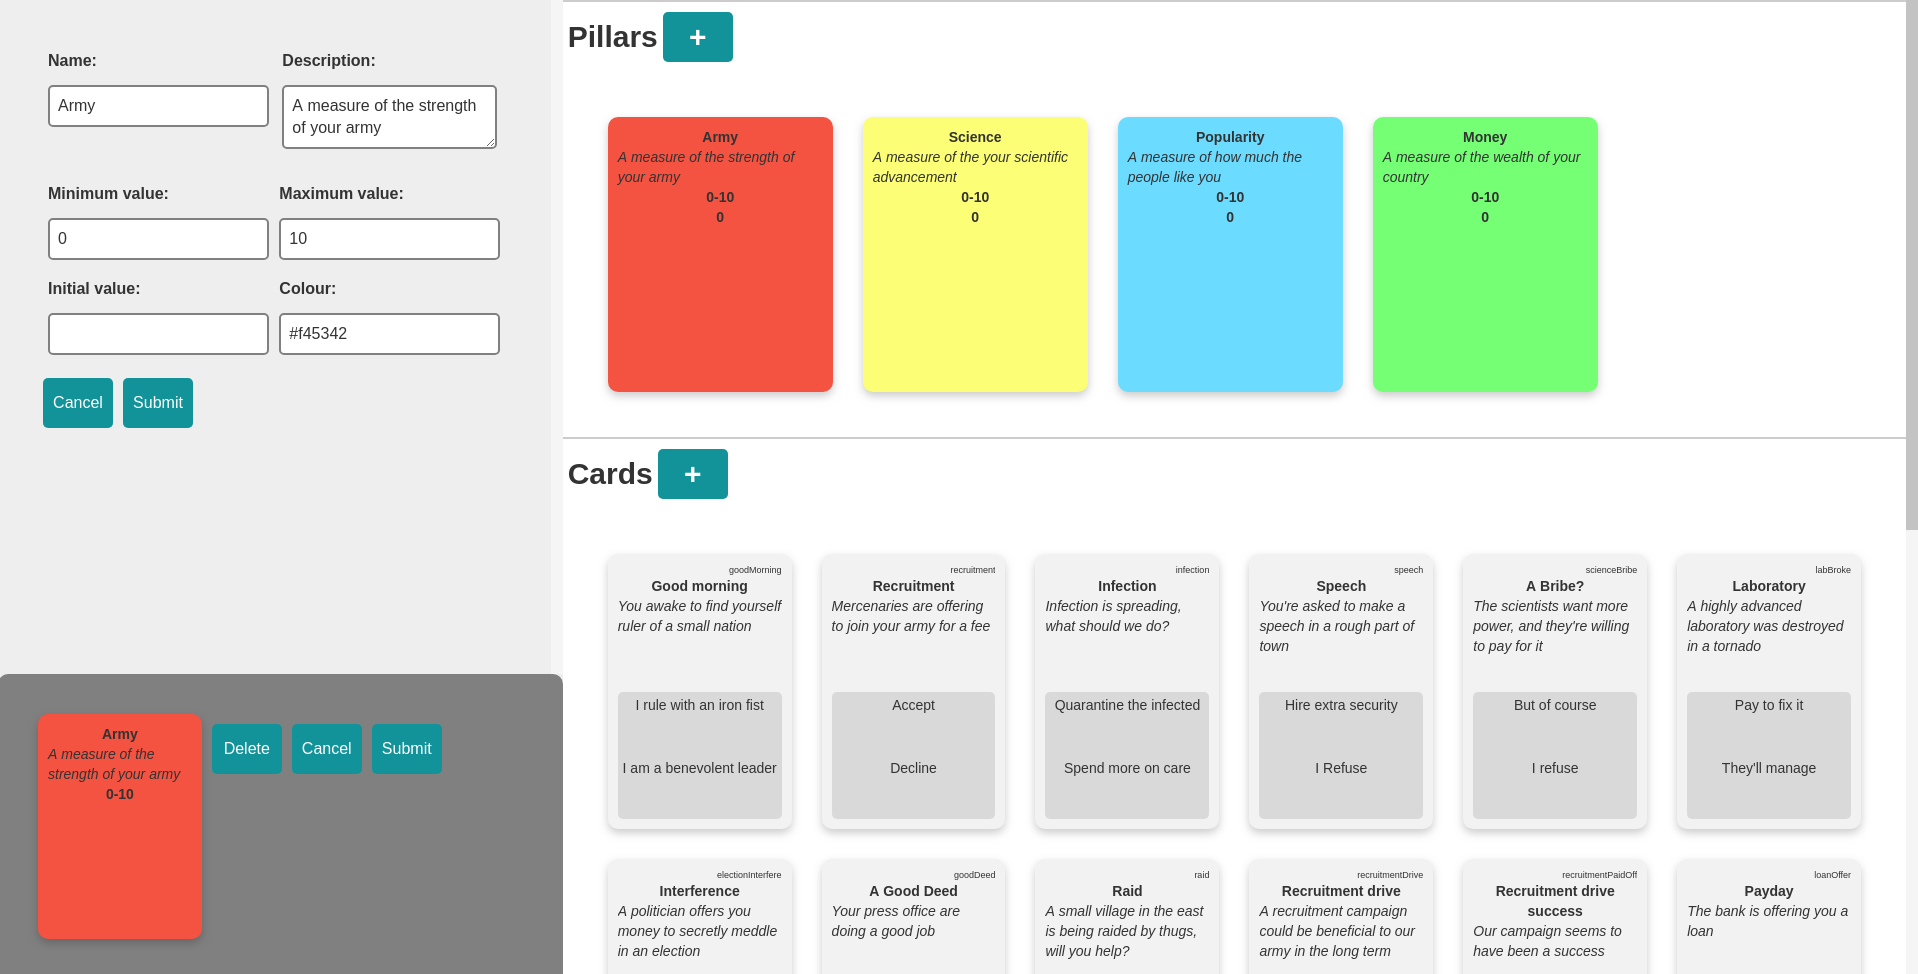
\includegraphics[width=1.0\textwidth]{./images/design/pillar_edit.png}
	\caption{Pillar editing view}
	\label{fig:pillar_edit}
\end{figure}

Clicking \c{Save Current} will save the updated game definition to the database, and it can then be played from the game UI by entering the correct game ID.

\subsubsection{Visualisation}
\todo[inline]{Discuss export}

The visualisation screen took a similar shape to the game maker, with data selection and filtering happening in a left panel while the visualisations are updated on the right.
It is possible to filter results to be visualised by pillar values. This limits the data shown only to cards that appeared while pillar values match the specified criteria The visualisations I chose to show are as follows:
\begin{itemize}
    \item Accept/Reject balance

    This is a horizontal bar chart showing the proportion of players that choose one option over the other for a given set of cards. Each card has a value between -1 and 1, where -1 indicates that players choose the reject option every time, while 1 indicates accept is chosen every time.

    \item Total times drawn
    
    This is a vertical bar chart showing the total number of times each card has been drawn and responded to.
    
    \item Pillar average

    This shows the average pillar levels over all turns.
\end{itemize}

The intention of these visualisations is to allow a user to `play' with the data. The live updating charts allow the user to rapidly identify relationships, for example between pillar levels and accept/reject balance.

\begin{figure}[!h]
	\centering
	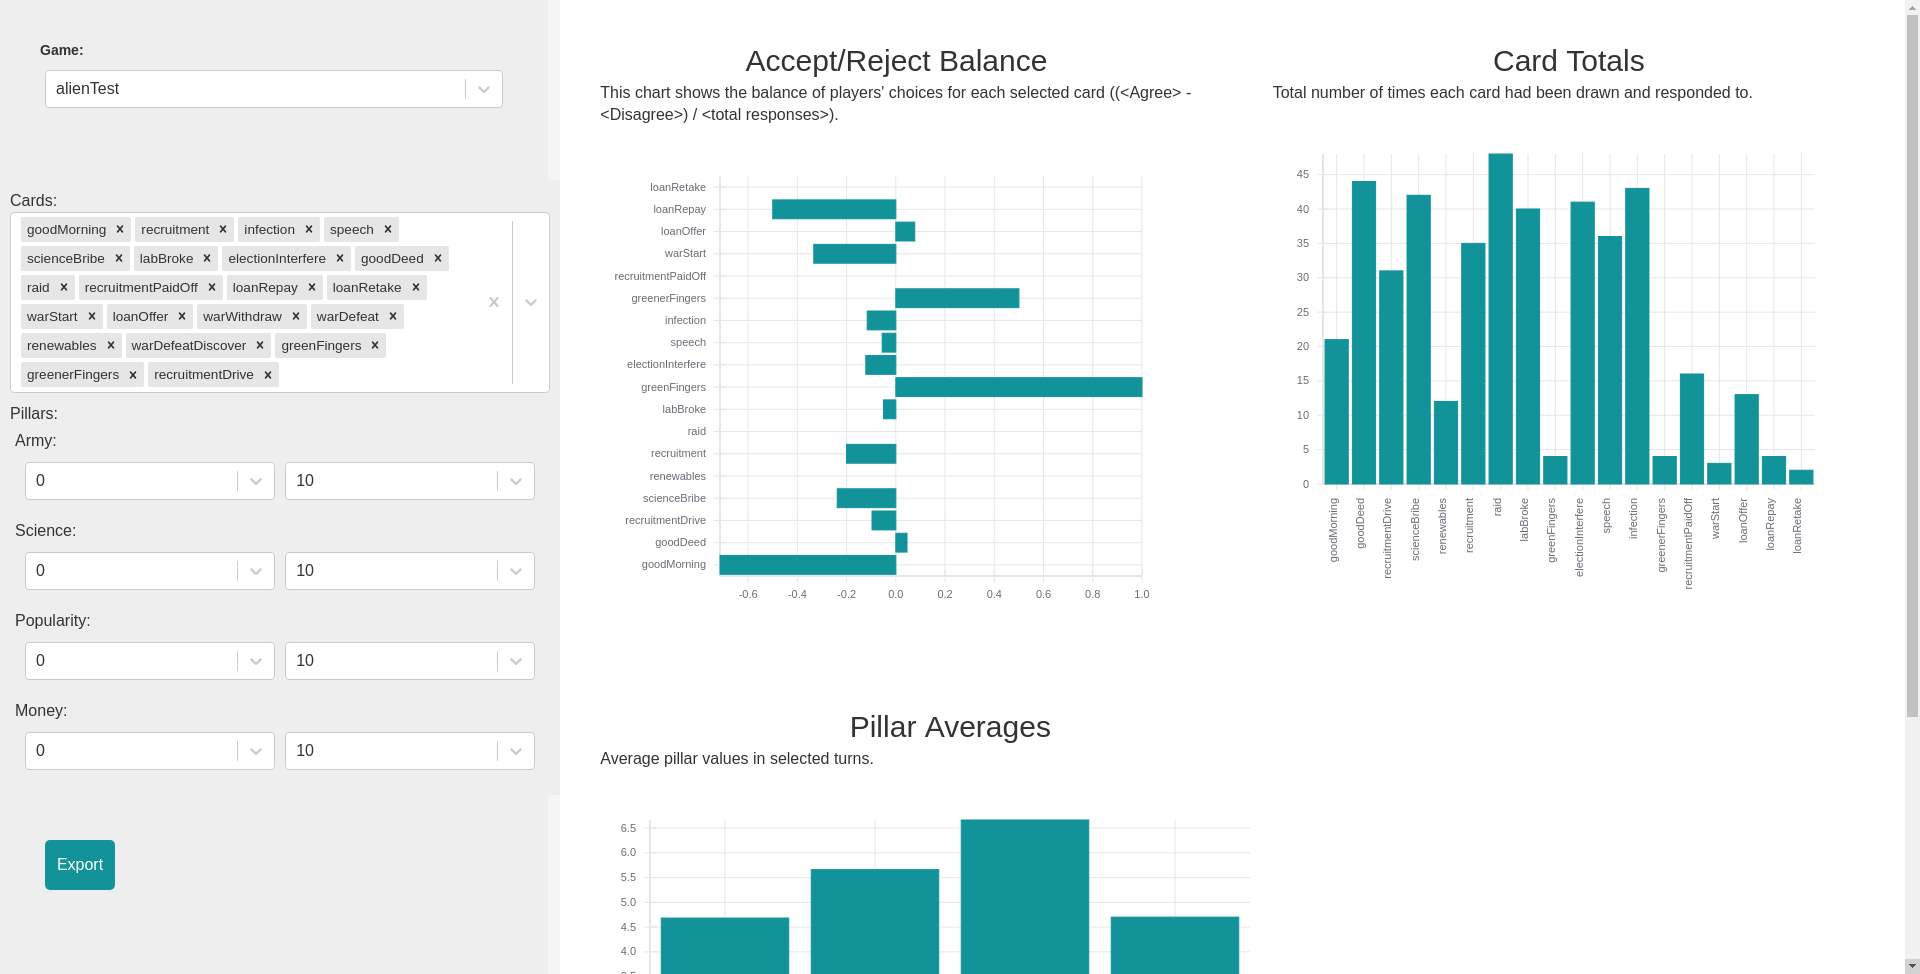
\includegraphics[width=0.45\textwidth]{./images/design/visualisation.png}
	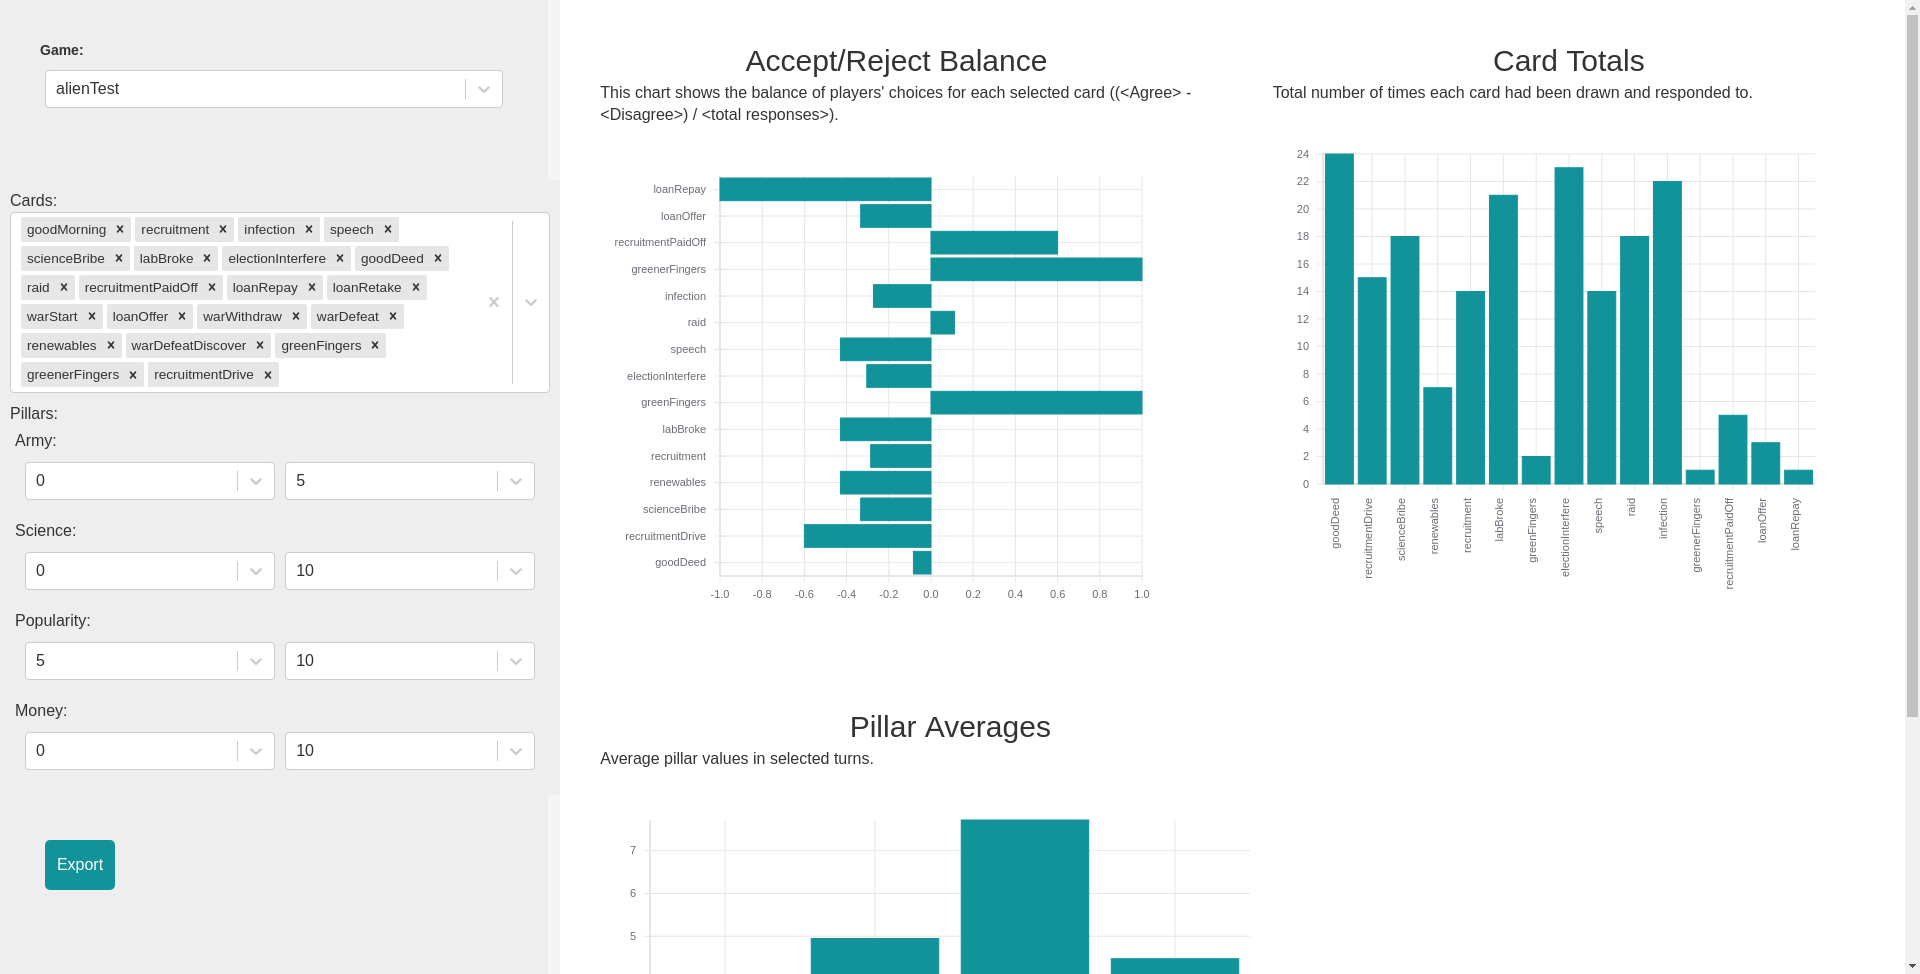
\includegraphics[width=0.45\textwidth]{./images/design/visualisation_filter.png}
	\caption{Visualisation screen effects of filtering data by cards and pillar values. This example filters responses to cards during turns where the player's \c{Army} was between 0 and 5, and their \c{Popularity} was between 5 and 10.}
	\label{fig:visualisation}
\end{figure}

The other function this page offers is the ability to export data to CSV. This effectively repackages the database as a csv file, where each row represents the turn of a user. Individual games are uniquely identified by sets of rows with the same user id and game id.

\section{Frontend}
When using Redux, one of the first design decisions that must be made is the structure of the Redux store. This is the JavaScript object that holds the page's state. Figures \ref{fig:store_shape} and \ref{fig:card_example} show a visual representation of the store for the game site. The game logic runs client-side, so to enable this, the entire game definition is requested from the database server once the player requests to play it. Depending on the use case, this could be considered a downside as technically a player could `cheat' the game through using console commands. This choice did however greatly simplify the API between the client and sever, as once the game has begun, the client only needs to send the outcome of each turn.

\begin{figure}[!h]
	\centering
	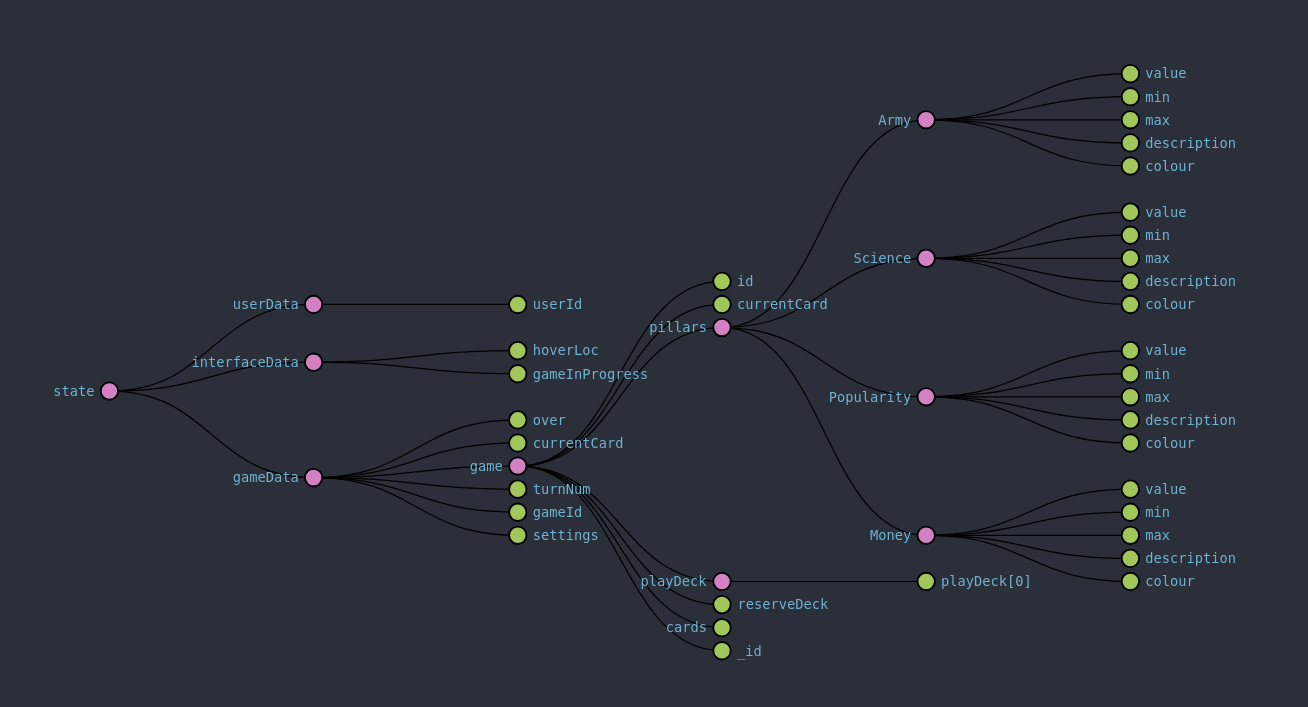
\includegraphics[width=1.0\textwidth]{./images/design/store_shape.png}
	\caption{Redux store object structure. Note that the pillars (Army, Science, Popularity, Money) are game definition dependent. Cards object is omitted due to large size.}
	\label{fig:store_shape}
\end{figure}

\begin{figure}[!h]
	\centering
	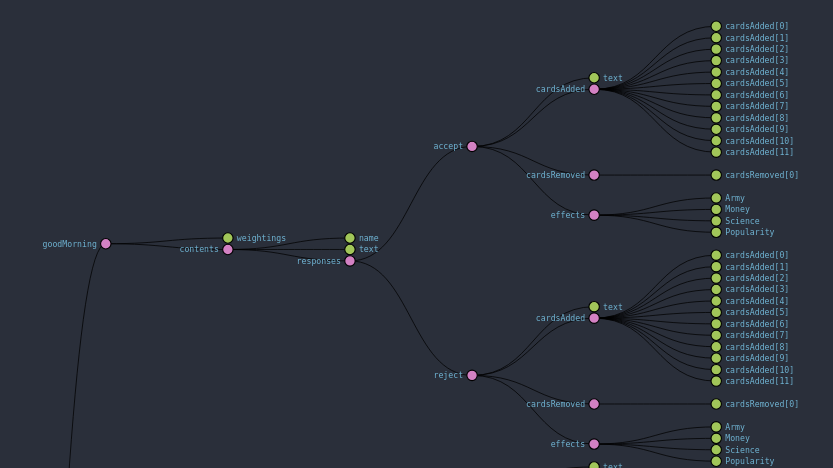
\includegraphics[width=1.0\textwidth]{./images/design/card_example.png}
	\caption{Example of a card object in the store. This is a starting card that adds many other cards to the game no matter which option is chosen.}
	\label{fig:card_example}
\end{figure}

\section{Backend}
Access to the database is provided through a backend server 
\chapter{Implementation}

\todo[inline]{Game workings}
\todo[inline]{Reducers}

\section{Tools \& Technologies}

\subsection{Node.js}
I decided early on that this application should be easily accessible on a range of devices, particularly the game interface. For this reason I built the system as a responsive web-application, running on a node server. Node\cite{Node} is an excellent framework for getting sizeable projects up and running very quickly, which I was able to do with this project. This is in part due to NPM\cite{npm}, which provides access to countless packages which I was able to use, ranging from Victory\cite{Victory} for visualisations, to Thunk\cite{Thunk} for managing asynchronous side effects.

\subsection{TypeScript}
According to Microsoft who maintain it, `TypeScript is a typed superset of JavaScript that compiles to plain JavaScript'\cite{Typescript}. 
I decided to use TypeScript (TS) to combat some of the problems that can occur when working on a large JavaScript codebase. 
Being statically typed, TS prevents type errors and instantly makes code more navigable and readable. 
This helps both during development and maintenance, which is particularly important if others continue to work on this project.

\subsection{TSLint}
Alongside TypeScript, I set up TSLint\cite{TSLint}, a linter for TypeScript. This was a huge help with development, as TSLint catches issues that can affect the performance of the application. For example, using arrow functions in JSX results in the function being recreated each time the component renders. This can then lead to the component re-rendering due to the shallow comparison of the old and new functions. This can lead to performance issues, which could have been troublesome for the more responsive parts of my software, such as the visualisation page. TSLint also provides general code cleanup features such as organising imports.

\subsubsection{React}
React\cite{React} is a UI library that simplifies the creation of responsive interface components. I knew that I wanted my application to be highly responsive, with each section effectively being split into a single page application. React made this fairly trivial once the structure of the page was settled, as information flows down through components and they are automatically updated.

\subsubsection{Redux}
Redux\cite{Redux} complements React nicely, by helping to manage state. When using pure React, each component stores it's own state. This can make things confusing as components that should be reflecting information can fall out of sync. Redux encourages moving the state of the whole application into one top-level serializable JS object. This then acts aas a `single source of truth', which takes care of several considerations. Another benefit that I found redux to have is the debugging tools, which take the form of a chrome extension\cite{ReduxDev}. When Redux is correctly used, this tool makes it possible to view and manipulate the application state, and even `time travel' the page to a previous state, such as before a button was clicked. This made debugging very straightforward, particularly for the game logic.

\begin{figure}[!h]
	\centering
	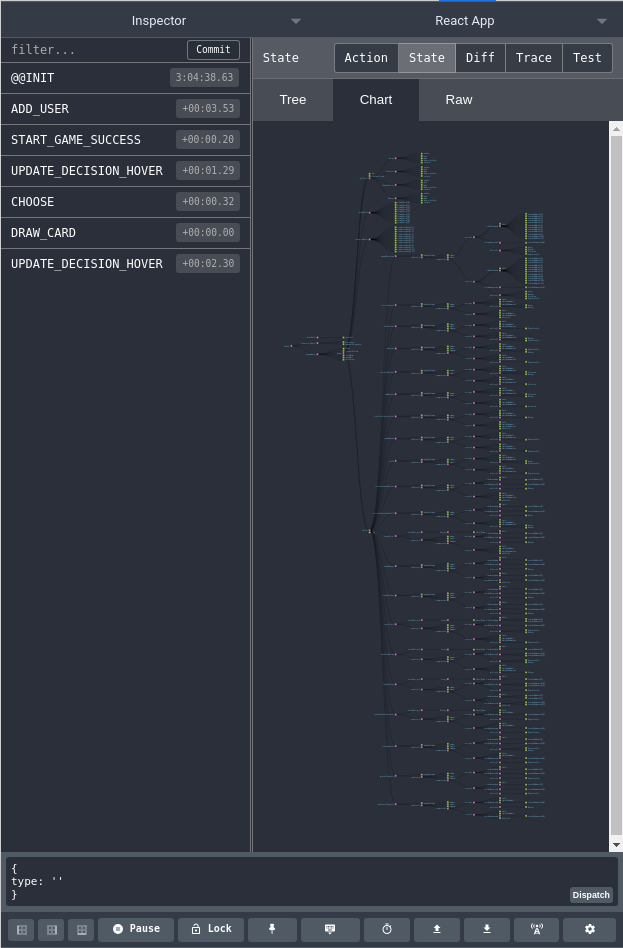
\includegraphics[width=0.8\textwidth]{./images/impl/redux_view.png}
	\caption{Redux DevTool\cite{ReduxDev} opened in game view. This shows what actions have occurred while the page has been open, as well as visualising the application state.}
	\label{fig:redux_view}
\end{figure}

\subsection{NeDB}
To store both the game definitions and the gameplay data, I needed a form of server-side persistance. I had  decide here between designing and maintaining a rigid relational database, or opting for a NoSQL\cite{NoSQL} solution. After consideration, I chose to go with a document-based database. The main factor in this decision was that I was unsure of what data would be desired by users of the final product. While a relational database requires strict definitions of data and their types, document-based databases are much more free form, meaning values can be added and removed with no alterations to the database server required.

Specifically, I chose to use NeDB\cite{NeDB}. NeDB is a lightweight JS database library that was quick and easy to set up and use. The API it provides is a subset of that of MongoDB\cite{MongoDB}, and was therefore well documented despite this being a smaller, more lightweight tool. Game definitions and user data are stored in two separate instances.

This database implementation does have some downsides in terms of long term maintenance - ideally further along in the project's life cycle this would probably be converted to a relational database, once the data requirements were more strictly defined. Also, regrettably NeDB does not expose encryption as part of its API.
This was something I only became aware of towards the end of the project, I might have chosen a different library if this had been immediately obvious. It would still be possible to encrypt fields individually
It did however suit the needs of the project, and I believe I made the right choice in getting started with NoSQL.

\section{Frontend}

\subsection{Game}

\subsubsection{Logic}
Most of the game logic happens in the redux reducers. 
This is the part of the code where actions arrive and the payload gets processed, resulting in some change to the game state which is then propagated through the page.

Reducers should technically be pure functions, as this makes them reliably testable and allows the time travel aspect of the debug tools to work correctly. 
I have followed this convention for all of my reducers, except for \c{CHOOSE}, which is called when the player makes a choice. 
This is because of the shuffle function that gets called, which has a random element.

The shuffle function I used is an implementation of the Fisher-Yates Shuffle\cite{Shuffle}. 
I needed this to ensure that the game remained unpredictable across replays, improving replayability.

Building the play deck is simply a case of iterating through each card that is out of play and adding those that match the requirements, as well as iterating through the previous play deck and removing those that do not.

\subsubsection{Images}
The colouring of images was one of the more technically involved parts of the project. 
In order to avoid heavily pixel processing I knew I would have to use SVGs, which can be edited with comparably insignificant computation (also having the advantage of being infinitely scalable). 
I then had to acquire some example images to use for my game definition. 
To maintain a similar art style I sourced them all from the same artist, Katerina Limpitsouni, on her site unDraw\cite{Undraw}. These images are open-source and usable for free and without attribution. 
The website has the advantage of allowing the main colour of each image downloaded to be set through a colour picker. 
After failing to find a solution to edit specific colours of an SVG in JavaScript, I resorted to wrapping each image in a React component, which passes through and injects the desired colour. 
This was not a favourable solution, as it's not possible to do this through the game maker tool. 
Considering this a prototypical feature (and not part of requirements), I believe the implementation is satisfactory.

Alternatively to this solution, another, less technically challenging but more time consuming possibility would be to fill the image URL property of each card, which could then be downloaded and rendered client-side.

\subsubsection{Hover}
When the user hovers over an answer with the mouse, the pillars affected by that response are outlined with a border, the colour of which depends on whether the effect is positive or negative. 
There were multiple ways in which this could have been implemented; I decided to use an enum property in the global state. 
Doing so makes it extensible - other effects or other hovering elements could be added easily.

\subsection{Game Maker}
Much of the time I spent working with CSS was on the game maker page, particularly the card and pillar views. 

Within the cards, if any text overflows beyond the limit of its section, it slowly fades out towards the bottom. This indicates to the user that there is more text to read, avoiding the situation where text is cut off but this is disguised by the gap between two lines of text. This effect is achieved by adding a fixed-height, partially transparent gradient matching the background colour to the bottom of each text \c{div}.

Cards are displayed in a responsive grid, which was done using CSS-flexboxes. I first used a combination of the \c{flex-basis}, \c{min-width} and \c{max-width} properties to allow each card to expand and contract slightly beyond its initial size. These were then placed inside a \c{div} with \c{display:flex}, allowing the cards to dynamically size and arrange themselves according to the size of this parent container. Using the Emotion\cite{Emotion} library, I was able to inject inline styles into the \c{hover} attribute of the card component, which allowed me to create the card expansion effect on hovering over them.

\todo{Responsiveness screenshots}

\section{Testing}
Thanks to the structure enforced by Redux, the application logic is entirely contained within one file - \c{reducers.tsx}. This simplifies testing, as the important code can be covered with a few well chosen unit tests. To write these tests I used Jest\cite{Jest} - a fairly simple JavaScript testing framework.
\chapter{Evaluation}
\todo[inline]{
'consider adding hidden columns which could affect the game but couldn't be seen by the user'
'only two answers per question?'
'subdecks - response can swap the whole deck eg when finding aliens'
    -can be done technically but easier
'Add/remove all UI element'}
\chapter{Conclusion}
Comparing my project to the software I found to be most like mine, Datagame \cite{Datagame}, I find that my software holds up well. I believe the game I have created is as engaging, if not more so than the games available on Datagame. Both game makers offer a similar toolset, and while I cannot speak for any analysis tools that Datagame provides, I believe the functionality provided by my analysis tools - combined with data export functionality - is sufficient. Is previoiusly stated, I cannot evaluate the accuracy with which the tool can infer player's opinions, however it may provide a point from which research into this area can proceed.

My game has achieved or surpassed the majority of my goals, and I feel confident that it could provide the grounds for further research into the world of gamification and opinion gathering.


\nocite{*}
\printbibliography
\end{document}
